\documentclass[output=paper]{langsci/langscibook} 

% font setting:
\newcommand{\textci}[1]{\textit{\textbf{#1}}}

\title{Aiming with → Arrows ← at
  Particles. Towards a Conceptual Analysis of Directional Meaning
  Components in German Particle Verbs}

\author{%
  Sylvia Springorum\affiliation{Institut für Maschinelle Sprachverarbeitung, Universität Stuttgart}\and 
  Sabine Schulte im Walde\affiliation{Institut für Maschinelle Sprachverarbeitung, Universität Stuttgart}
}

% \chapterDOI{} %will be filled in at production

% \epigram{}

\abstract{This article presents a case study on the contributions of
  prepositional particles to the meanings of German particle verbs
  (such as \textit{anstrahlen} `to beam/smile at' and
  \textit{aufgeben} `to give up'). Based on a set of 16 ``concept
  images'', two-dimensional directional arrow pictographs, 60
  experiment participants selected one or more concept images for a
  systematically composed set of 270 German particle verbs and their
  30 base verbs. We formulate a series of hypotheses for the meanings
  of nine constituent particle types (\textit{ab, an, auf, aus, ein,
    mit, nach, vor, zu}) and investigate them in the light of the
  concept image selections. Qualitative and quantitative analyses
  indicate that our hypotheses are largely confirmed, across three
  source domains varying in their abstractness (\texttt{Machines \&
    Tools, Force, Sound}), as well as across well-known vs. unknown
  particle verbs. The particles exhibit individual concept image
  profiles, and they vary in their flexibility to provide predominant
  directions; for example, while \textit{auf} is rather consistently
  perceived as contributing an upward right direction to a particle
  verb meaning, \textit{an} shows similarly strong preferences for a
  set of concept images; in both cases, these tendencies are observed
  across source domains.}


\begin{document}

\maketitle


\clearpage
\section{Introduction}

German particle verbs (PVs) are complex verb structures such as
\textit{anstrahlen} `to beam/smile at' that combine a prefix particle
(\textit{an}) with a base verb (\textit{strahlen} `to
beam').\footnote{German distinguishes between separable particle verbs
  and non-separable prefix verbs. Our focus is on particle verbs.} PVs
represent a type of multiword expressions, which are generally known
as a \textit{``pain in the neck for NLP''} \citep{SagEtAl:02}. Even
more, German PVs pose a specific challenge, because the particles are
highly ambiguous; e.g., the particle \textit{an} has a partitive
meaning in \textit{anbeißen} `to take a bite', a cumulative meaning in
\textit{anhäufen} `to pile up', and a topological meaning in
\textit{anbinden} `to tie to' \citep{Springorum:11}. In addition, the
particles often trigger meaning shifts of the base verbs (BVs),
cf. \citet{SpringorumEtAl:13,FrassinelliEtAl:17,Koeper/SchulteImWalde:18,SchulteImWaldeEtAl:18};
e.g., the PV \textit{abschminken} with the BV \textit{schminken} `to
put on make-up' has a literal meaning in a concrete context (`to
remove make-up'), as in example~(\ref{ex:abschminken1}), and a
metaphorical meaning in an abstract context (`to forget about
something'), as in example~(\ref{ex:abschminken2}).

\ea\label{ex:abschminken1}
\gll Den Lippenstift kannst Du Dir abschminken.\\
the lipstick can you yourself {[ab] put on make-up}\\
\glt `You can remove the lipstick.'
\z

\ea\label{ex:abschminken2}
\gll Den Job kannst Du Dir abschminken.\\
the job can you yourself {[ab] put on make-up}\\
\glt `You can forget about the job.'
\z

% Particle verbs constitute a significant part of the verb lexicon
% \citep{Koeper:18}.  For example, the German web corpus DECOW14AX
% \citep{Schaefer/Bildhauer:12,Schaefer:15} with a total of 12 billion
% words includes ca. 7,000 different PV types. In comparison, the number
% of BVs is 5,000.
%
% SIW: Zahlen sind aus
% /projekte/semrel/Resources/Corpora/COW/COW-de14AX/windows-pv-corrected bzw. 
% /mount/arbeitsdaten29/corpora/waterloo/pv_data/1LineDecow14AX_MC100.gz.

Not only the particle types but also the particle verbs as a whole
often have more than a single reading. For example, the PV
\textit{anstrahlen} not only means `to beam at' but also `to smile
at', when derived from the metaphorical meaning of \textit{strahlen}
(`to beam'), i.e. `to smile'. The PV \textit{abnehmen} not only means
`to take off/away', but can also be used to express `to reduce' as an
incremental interpretation of `to take off/away'; in addition, it has
obtained the specific sense `to reduce weight'. The semantic
decomposition in the latter two examples seems to be less transparent
than in the previous ones, thus indicating different degrees of PV
compositionality. Accordingly, we also find opaque compositions such
as \textit{aufhören} (`to stop'), where the semantics of the BV
\textit{hören} (`to hear') does not seem to provide any contribution
to the PV meaning at all. Such examples are the reason why PV
composition is often deemed idosyncratic, cf. \cite{Kratzer:03}.

In this chapter, we explore the meaning contribution of particle types
to the meanings of German particle verbs across three semantic domains
of base verbs, which vary in their degree of abstractness:
\texttt{Machines \& Tools, Force, Sound}. Within our study, we focus
on prepositional particle types and the role of directionality. In
this vein, Section~\ref{sec:p-meaning} will motivate our assumptions
about particle meanings in German PVs in more detail, before
Section~\ref{sec:exp} presents the design, hypotheses and results of
an experiment that collected human judgements on directionality in
particle meanings. Section~\ref{sec:2discussion} discusses the
experiment data and reflects on our preceding assumptions about
prepositional particle meanings.


\section{Particle meanings}
\label{sec:p-meaning}

\subsection{Basic particle meanings and contexts}

For the course of this article, we assume that each particle type has
a restricted number of simple primary meanings, which we refer to as
\textit{basic meanings}. This is in accordance with \cite{Lindner:83},
who identifies a prototypical sense for the English verb particle
\textit{out} involving `paths in the spatial domain'. Without a BV
context, the basic particle meanings are underspecified first, and
then resolved by contextual constraints provided by the BV. For
example, the separation introduced by the particle \textit{ab} in the
context of the BV \textit{nehmen} (`to take') evokes a change of state
`to take off/away', whereas in the context of the BV
\textit{schminken} (`to put on make up') it evokes a duration `to
remove make up' generated by a sequence of separations. However, not
only the BV but also further context has to be taken into account, as
there are ambiguous PVs with varying particle meaning
contributions. For example, regarding the metaphorical meaning of
\textit{abschminken} in example~(\ref{ex:abschminken2}), \textit{ab}
introduces only a single separation event, in contrast to the sequence
of separation events in the literal PV reading.

Previous research has pointed out regularities in the interpretation
of particle meanings associated with semantically coherent classes of
base verbs,
cf. \cite{Stiebels:96,Lechler/Rossdeutscher:09,Kliche:11,Springorum:11}.
For example, \textsc{Direction} and \textsc{Contact} represent two
independent readings of \textit{an}, among others: The PV in
example~(\ref{ex:anschauen1}) belongs to the \textsc{Direction}
meaning class, suggesting that \textit{an} assigns a direction to the
BV, whereas in example~(\ref{ex:ankleben}) the PV carries a
\textsc{Contact} particle meaning. In combination with a movement BV
as in example~(\ref{ex:anfahrenLaterne1}), the particle again
introduces a direction. In addition, the meaning of \textit{anfahren}
requires a decreasing distance, which results in a contact when
maximal. Therefore, \textit{anfahren} represents an example with
meaning components from both classes, \textsc{Direction} and
\textsc{Contact}. Examples~(\ref{ex:anschauen1})--~(\ref{ex:anfahrenLaterne1})
show that particle senses vary in their complexity, and they also
illustrate the limits of a hard class assignment.

\ea\label{ex:anschauen1}
\gll Karin schaut das Bild an.\\
Karin look the picture [an]\\
\glt `Karin looks at the picture.'
\z

\ea\label{ex:ankleben}
\gll Karin klebt die Briefmarke an.\\
Karin stick the stamp [an]\\
\glt `Karin sticks on the stamp.'
\z

\ea\label{ex:anfahrenLaterne1}
\gll Karin fährt die Laterne an.\\
Karin drive the lantern [an]\\
\glt `Karin drives against the lantern.'
\z

In addition, a classification of PVs should not only take lexical
information into account. Sentimental connotations, associations to
other sensory input, (nature) forces, and dimensionality are just as
well involved in the process of sense development. For example, the
metaphorical PV \textit{abklappern} (lit. [ab]+`to clatter')
illustrates that sensory information can be understood as a part of
the PV meaning: \textit{abklappern} creates an ideophone, which is
mapped to the verb event, and leads to the meaning-shifted sense `to
pursue something successively', as illustrated by
example~(\ref{ex:abklappern}). This perception-based meaning shift
process is discussed in more detail by \cite{SpringorumEtAl:13}.

\ea\label{ex:abklappern}
\gll Sie klapperte die Geschäfte nach tollen Büchern ab.\\
she clattered the shops for great books [ab]\\
\glt `She successively searched through the shops for great books.'
\z

Particle meaning is not only influenced by its context, but also
provides an influence on the meaning of the context. For example,
participants in a sentence generation experiment relying on
systematically created PV neologisms (neoPVs) were asked to generate
sentences for neoPV types such as \textit{antöten} ([an]+`to kill')
and \textit{abschlafen} ([ab]+`to sleep'), without being provided any
context \citep{SpringorumEtAl:13cALTER}. The participants did not only
show considerable agreement regarding potential neoPV meanings, but
also often agreed in their strategy of dealing with particle senses,
in cases where the BV meaning did not fit to the PV senses, as in the
case of \textit{antöten}, where `to kill' introduces an absolute
change of state, and the generated sentences mainly suggested an
\textit{an} meaning of \textsc{Partial Affectedness}, thus introducing
quantification over event parts. This meaning typically cannot be
applied to a verb with an absolute change of state, such as
\textit{töten}, but the participants obviously re-conceptualised the
change-of-state BV \textit{töten} as a process verb, which gradually
approximates the final state of death. Often, adverbial specifications
such as \textit{fast tot} (`nearly dead') were added, which supported
the above assumptions. The meaning components in the PV based on the
BV were thus adjusted dependent on the particle meaning.

In sum, we define the meaning of a PV as either a direct composition
of possible meaning components of particle and BV (if they are
compatible), or alternatively as meaning-shifted particle and BV
meaning components in strong interaction with the context. On the one
hand, PVs can be assigned to discrete particle classes, based on
semantically coherent groups of BVs, but on the other hand the classes
need to be flexible, to allow semantic changes if necessary. At first
these two alternative options might seem contradictory, but from a
diachronic perspective they reflect two natural processes of sense
development. For example, according to \cite{Waldron:79} ``new words
should first be used in rather specialised senses and subsequently be
generalised'' and ``when such words have once achieved general status
we use them without reflection upon their former restricted or
technical sense''. In addition, ``the reverse process, in which a
general word is given a special meaning in a restricted context, is
just as common''. In this sense, the polysemy of particles is
considered as a result of adjustment processes of basic meanings to
recurring contextual conditions.

\subsection{Spatial grounds of particle meanings}

As we are focussing on PVs with prepositional particles, we assume
that particles are spatially grounded, similar to preposition
meanings. Prepositions indicate spatial fundamentals, as discussed by
\cite{Herskovits:86} and \cite{Dirven:93}, among others. They
structure the physical space and determine ``language-specific
concepts built up in mental space''. Simlarly, \cite{Gaerdenfors:04}
claims that prepositions are ``primarily spatial relations'' and
create ``spatially structured mental representations'', when used with
non-locational words. In order to structure space, it has to be
perceived through our senses, with vision representing the predominant
human sense \citep{Viberg:83}.

Furthermore, \cite{Jackendoff:83} understands ``perception as an
interaction between environmental input and active principles in the
mind, that impose structure on that input''. He demonstrates his view
by ambiguous pictures from the school of Gestalt psychology.
\cite{Lakoff:87} refers to the ``spatialisation of form hypothesis''
by using the term \textit{Image Schema}, which he defines as
``schematic descriptions of meaning concepts''. So perception of space
cannot be separated from cognitive conceptualisation, and (meaning)
concepts are often analogies of structures, to define space through
perception. Although there are ``significant differences between
mental imagery and Image Schemas'', according to
\cite{Gibbs/Colston:95} there is ``good evidence that both spatial and
visual representations exist for mental imagery''.

We assume that prepositional particles --simlarly to prepositions--
introduce relations to structure space and to add verb-related meaning
components, such as aspectual or temporal modifications. These
relations can be captured by Image Schemas as ``dynamic analogue
representations of spatial relations as movement in space''
\citep{Gibbs/Colston:95} to describe aspects of PV
meaning. Accordingly, earlier investigations connect (spatial)
concepts with phrasal verbs. Going beyond the already mentioned work
by \cite{Lindner:83}, \cite{Morgan:97} provides an extension for
metaphorical readings of some \textit{out} phrasal verbs. From a
didactic point of view, \cite{Side:90} and \cite{Abreu/Vieira:08}
discuss the advantages of using Image Schemas in order to learn
phrasal verbs. In a psycholinguistic setting, \cite{RichardsonEtAl:01}
carried out experiments to show that basic images can be related to
spatial and abstract verbal meanings.

A semiotic perspective of schematic descriptions is provided by
\cite{Frutiger:87}, who defines the essential task of a schema as
description with the help of literally pictured elements, to divide
objects into different parts, instead of only using
words. \cite{Neurath:83} developed the international picture language,
which is based on pictographs instead of words, as a complementary
system to natural language, because in some cases pictures or
pictographs are better in transmitting information, as they are more
universal than words. Such pictographs transmit conceptual information
and therefore act on a universal level. They meet our demands to
describe basic particle meaning components, both context- and
domain-independent.


\section{Experiment}
\label{sec:exp}

This section presents the material, design, hypotheses and results of
the experiment that collected human judgements on spatial aspects in
particle meanings.

\subsection{Material}

\subsubsection{Verb data}
\label{sec:data}

The German particle verbs for the experiment were generated
systematically, based on a pre-selected set of base verbs and a
pre-selected set of particles. We relied on base verbs from three
different semantic domains, \texttt{Machines and Tools (MnT)},
\texttt{Force} and \texttt{Sound}, which differ regarding their degree
of concreteness. Furthermore, \cite{Koevecses:02} categorises
\texttt{MnT} and \texttt{Force} domains as common source domains for
metaphors. The verbs belonging to the \texttt{MnT} domain (such as
\textit{hämmern} (`to hammer') and \textit{schaufeln} (`to dig')) are
easy to imagine and represent very concrete BVs. In comparison, the
verbs from the \texttt{Force} domain (such as \textit{drücken} (`to
press') and \textit{quetschen} (`to squeeze')) are less concrete, as
the force itself is not perceivable directly, but only through
interactions of its concrete entities encoded in the verb
arguments. The verbs from the \texttt{Sound} domain (such as
\textit{schreien} (`to cry') and \textit{jaulen} (`to yowl'))
represent intransitive verbs and define the most abstract source
domain.

For each of the three domains we chose a total of ten base verbs that
we thought as not obviously ambiguous among the three classes, cf. the
Appendix. These 30 BVs were then systematically composed to PVs using
nine different prepositional particles. We only took into account
particles that cannot also be used in German prefix verbs: \textit{ab,
  an, auf, aus, ein, mit, nach, vor, zu}. In this way, we obtained 300
verbs (30 selected BVs and 270 generated PVs) as target verbs for the
experiment. Due to the systematic composition of the PVs, also PV
neologisms (neoPVs) were part of this data set. As part of the
experiment tasks, the experiment participants were thus asked to rate
a PV as a neologism, such that our analyses can distinguish between
existing PVs vs. PV neologisms. Approximately half of the PVs were
rated as neoPVs (153 out of 270 PVs), cf. Section~\ref{sec:design}
below.


\subsubsection{Concept images}
\label{sec:image-schema}

Although there are many semantic analyses based on concepts and
frequently illustrated by visual schemas or pictographs, as to our
knowledge there is no general systematic standard available. We
therefore decided to define visual representations for directional
concepts from scratch. As source for inspiration, we relied on
Dreyfuss' symbol sourcebook, a very detailed collection of various
kinds of symbols from many different areas \citep{Dreyfuss:84}, and on
a more descriptive sign derivation in \cite{Frutiger:87}. We defined
the set of directional pictographs as shown in
Figure~\ref{fig:CIdir}. The pictographs were intended to be as simple
as possible, to not distract from the actual information, but at the
same time they should allow possibly alternative interpretations. We
refer to our simplified pictographs as ``concept images''.

\begin{figure}[htbp]
  \vspace{+2mm}
  \caption{Set of concept images.}
  \label{fig:CIdir}
%  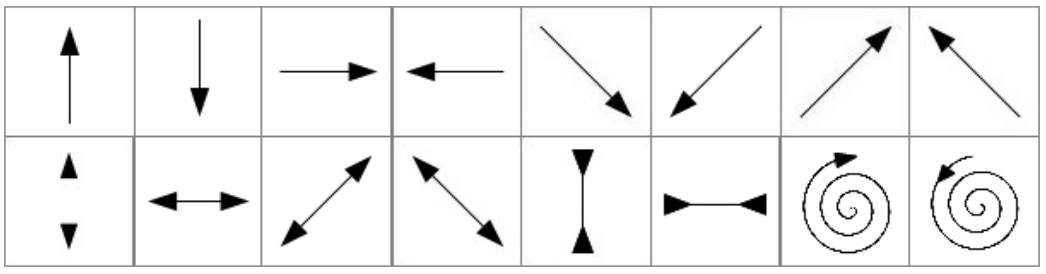
\includegraphics[width=.9\linewidth]{figures/CI-set}
  \hspace*{+1mm}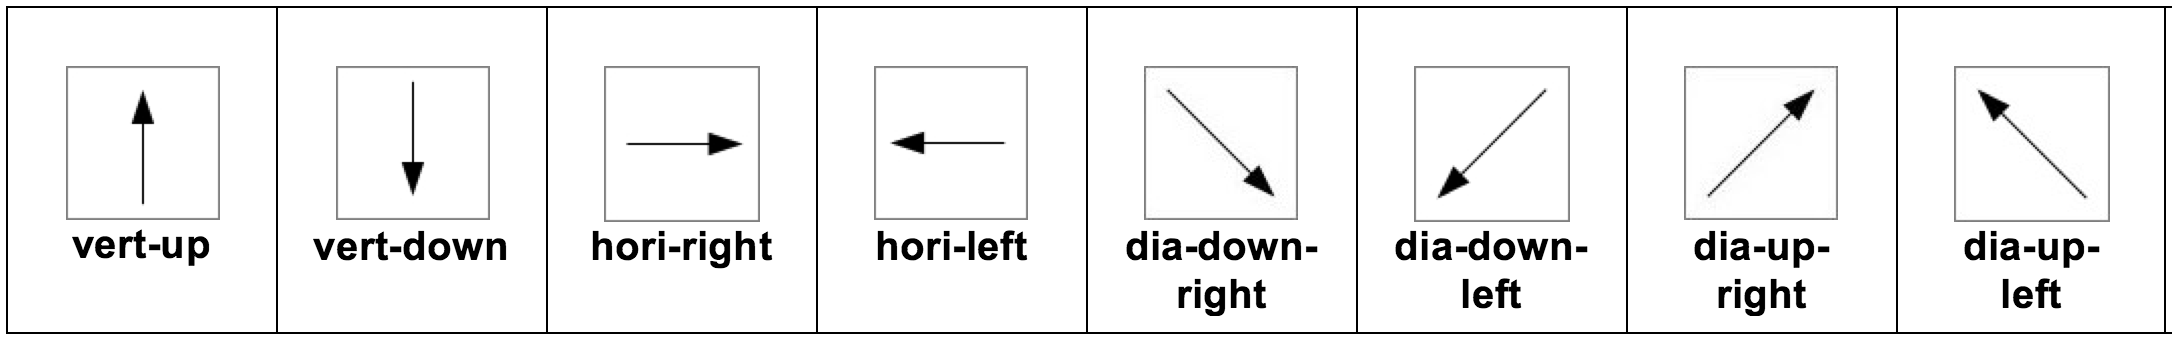
\includegraphics[width=.95\linewidth]{figures/CIs-1-8.png}
  \vspace{+3mm}\\
  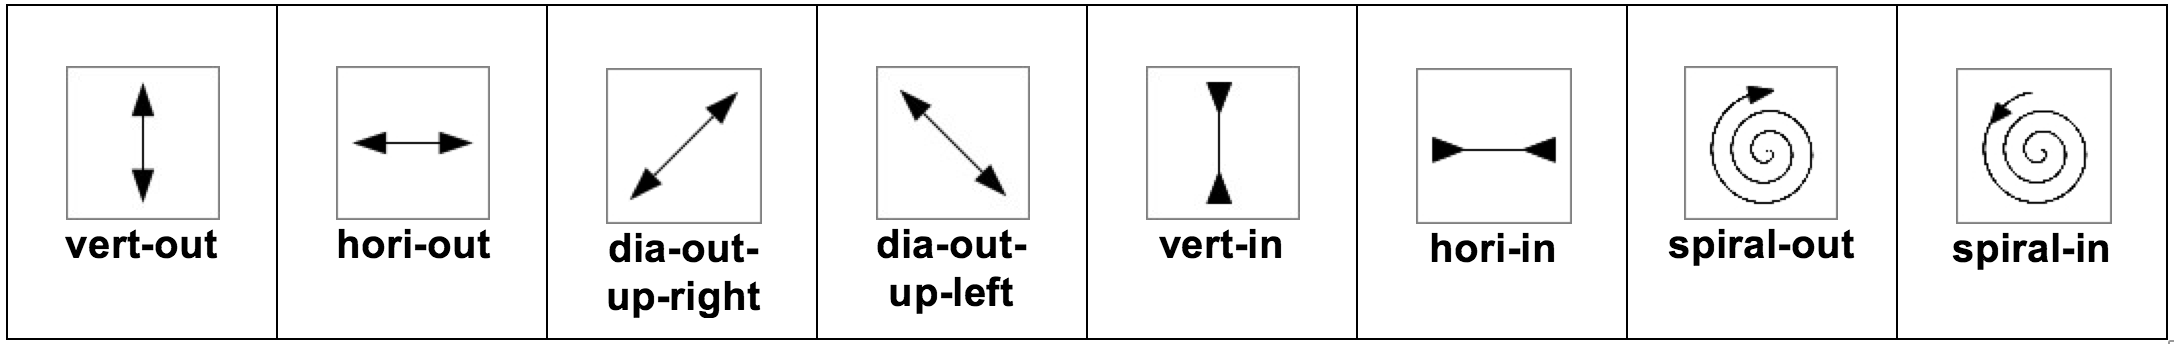
\includegraphics[width=.95\linewidth]{figures/CIs-9-16}
\end{figure}

Although the number of directions in space is infinite, a simplified
conceptual reduction into a two-dimensional setting is in many cases
sufficient, because ``the salient dimensions of the world reinforce
the horizontal and the vertical'' \citep{Tversky:11}. We therefore
included vertical arrows for upward and downward directions
(\textci{vert-up, vert-down}), horizontal right and left directions
(\textci{hori-right, hori-left}), and also the four diagonal
directions (\textci{dia-down-right, dia-down-left, dia-up-right,
  dia-up-left}). To represent single object-oriented center-periphery
directions as expansion or constriction, lines with arrow heads at
both ends are used. Whereas the outward-pointing arrow heads
(\textci{vert-out, hori-out, dia-out-up-right, dia-out-up-left})
correspond to expansion, the inward-pointing arrow heads
(\textci{vert-in, hori-in}) correspond to constriction. To distinguish
between asymmetrical and uniform center-periphery directions, two
arrows with concentric curved lines were added (\textci{spiral-out,
  spiral-in}). The total set of concept images contains 16 pictograms.


\subsection{Design}
\label{sec:design}

The experiment was performed as follows: The 300 verbs were
distributed randomly over 6 lists with 50 verbs each. The random
distribution was balanced for BVs vs. PVs, BV source domain, particle
type and (non-)neologism\footnote{At this point, we did not yet have
  human ratings for PV neologisms, so we used a pre-categorisation
  which considered a PV as neoPV if it did not appear in the
  \textit{SdeWaC} web corpus containing 880 million words
  \citep{Faass/Eckart:13}.}, such that each file contained equal
proportions of these.

Each verb was judged by $\approx$20 participants, non-experts (mostly
students on campus), without payment. They were presented a randomly
ordered list of the target verbs (printed out or as a file), together
with the concept images. For each verb, the participants were first
asked to choose between one of the following statements, to check on
whether they knew the PVs:
\begin{enumerate}
  \itemsep -1mm
\item unknown and difficult to understand;
\item unknown but easy to understand;
\item infrequent usage but known;
\item frequent usage and known.
\end{enumerate}
These ratings provided a participant-dependent categorisation of PVs
(and also of BVs, but those were not relevant for us) into existing
PVs vs. PV neologisms on a four-point scale.

Then the participants were asked to mark those concept images which
fit to the meaning of the target verb. Multiple marks were allowed
while we did not explicitly allow the participants to not select any
concept image because we wanted to enforce a selection. However, we
offered the participants to describe an alternative image if they
decided that none of our concept images fits. In that way they would
only fall back to not provide any selection if they really could not
settle on a concept image.


\subsection{Hypotheses}

The main goal of our study was to investigate whether prepositional
particles within German particle verbs can be associated with
directional concepts, which are visually represented as concept
images. As the basis for interpreting the experiment results, this
section provides example-based and experience-driven hypotheses for
the above-mentioned nine particle types regarding their most prevalent
readings. Regarding the particles \textit{ab, an} and \textit{auf}, we
in addition rely on detailed formal semantic analyses
\citep{Lechler/Rossdeutscher:09, Kliche:11,Springorum:11}.

Further than discussing the primary concepts as originating from the
spatial domain, we also include time into the interpretation of space,
as ``knowledge of space frequently comes from motion in time, from
exploring environments and piecing together the parts''
\citep{Tversky:11}. Furthermore, relying on \cite{Boroditsky:01}, who
analyses time with the help of spatial metaphors, ``concepts of space
appear to be primary'', concepts of time can be derived from concepts
of space.

\vspace{+1mm}
\subsubsection{\textit{ab}}

\textit{ab} has a basic meaning derived from the gravity force that
causes objects to fall. This motion describes a \textsc{Down}
directional meaning which may be represented by the concept image
\textci{vert-down}. An example is the particle verb \textit{ablaufen}
(`to run down') in example~(\ref{ex:ablaufen}) where the downward
meaning can only be contributed by the particle and not by the BV
\textit{laufen} (`to run'). In contrast, example~(\ref{ex:absinken})
with \textit{absinken} (`to sink')
% and in example~(\ref{ex:abfallen1}) with \textit{abfallen} (`to fall off'),
the event of the BV \textit{sinken} (`to sink')
% and \textit{fallen} (`to fall')
already introduces a downward direction. The difference between the BV
and the PV meanings is that the BV events refer to an atelic
continuous downward motion, as arising from the gravity force
\textsc{Down} direction, while the PV event is resultative, so a
direction is spanned between the pre-state and the resulting state of
the object affected by the gravity force. That is, in
example~(\ref{ex:absinken}) the pre- and result states are the
locations of the ship before and after the sinking motion. The PV
meaning is thereby almost synonymous to the BV meaning, which only
describes the downward motion of the ship, and in addition introduces
a result state.

\ea\label{ex:ablaufen}
\gll Das Wasser läuft ab.\\
the water runs [ab]\\
\glt `The water runs off.'
\z

\ea\label{ex:absinken}
\gll Das Schiff sinkt ab.\\
the ship sink [ab]\\
\glt `The ship sinks.'
\z
  
The PV \textit{abfallen} in example~(\ref{ex:abfallen2}) also
describes a downward direction with pre- and result states, regarding
the button affected by gravity. Here we however find a further meaning
component: the detachment of the button, a mereological part of the
jacket, has to be caused by some force. This
example~\ref{ex:abfallen2} suggests that the particle \textit{ab} may
also contribute a \textsc{Separation} meaning, which is --according to
previous lexical semantic analyses-- a productive reading for this
particle \citep{Kliche:11}. Often, it is not gravity but other
intentional forces which are causing detachments, as in
example~(\ref{ex:abreissen}) with the PV \textit{abreißen} (`to pull
off'). Here, the direction related to the force may even overwrite the
basic downward direction of \textit{ab}, which means that the particle
only contributes the \textsc{Separation} meaning component to the
PV. The directions are explicitly specified through the semantics of
the BV, through further contextual clues, or remain unspecified as in
example~(\ref{ex:abreissen}). In addition to the gravity-dependent
default direction described by \textci{vert-down}, a ``neutral'',
gravity-independent horizontal direction described by
\textci{hori-right} or \textci{hori-left} might therefore represent an
alternative choice of concept image.

\ea\label{ex:abfallen2}
\gll Der Knopf fällt von der Jacke ab.\\
the button fall off the jacket [ab]\\
\glt `The button falls off the jacket.'  
\z

\ea\label{ex:abreissen}
\gll Karin reißt den Knopf von der Jacke ab.\\
Karin pull the button off the jacket [ab]\\
\glt `Karin pulls the button off the jacket.'
\z

The continuous variant of the discrete \textsc{Separation} reading is
the \textsc{Decrease of Proximity} reading which occurs with motion
verbs as in example~(\ref{ex:abfahren}). Here the alignment with the
conceptual direction of time becomes obvious. Similarly, in sentences
as in example~(\ref{ex:absitzen}) with \textit{absitzen} (`to
wait/endure', lit. `to sit off') in an abstract context, the spatially
grounded basic concept has to be transferred to available abstract
dimensions, which are different from space. Regarding
\textit{absitzen}, the abstract context \textit{seminar} belongs to
the time domain, so that the direction of the particle \textit{ab} can
conceptually only align with the conceptual orientation of the time
dimension. The conceptual direction is thereby spanned between the
starting point and an iteration of separations of mereological parts,
which are time intervals. This leads to a \textsc{Progress} reading
which may be combined with a conceptually vertical value scale
\citep{Tversky:11} to a \textsc{Value Decrease} meaning, as in
example~(\ref{ex:abwerten}). Combining the \textsc{Progress} and the
\textsc{Value Decrease} dimensions, \textci{dia-down-right} is another
concept to be expected for the particle \textit{ab}. This idea is
comparable to \cite{Talmy:00}'s force dynamics, a conceptual notion of
forces split up into different components and relations, which can be
applied to various domains.

\ea\label{ex:abfahren}
\gll Karin fährt (von Stuttgart) ab.\\
Karin drive from Stuttgart [ab]\\
\glt `Karin departs (from Stuttgart).'
\z
  
\ea\label{ex:absitzen}
\gll Karin sitzt das Seminar ab.\\
Karin sits the seminar [ab]\\
\glt `Karin endures the seminar.'
\z
  
\ea\label{ex:abwerten}
\gll Karin wertet (mit ihrer Kritik) alles ab.\\
Karin values with her criticism everything [ab]\\
\glt `Karin devaluates everything (with her criticism).'
\z

\vspace{+1mm}
\subsubsection{\textit{an}}

\textit{an} introduces a direction which is force-independent in its
primary meaning, as in example~(\ref{ex:anschauen}), repeated from
example~(\ref{ex:anschauen1}), with the PV \textit{anschauen} (`to
look at') derived from the perception BV \textit{schauen} (`to look')
in a spatial context. The direction of human sight --with a neutral
head position which is horizontal by default-- determines this
conceptual direction. Given this, \textit{an} can be represented by
the concept images \textci{hori-right} and \textci{hori-left}.

\ea\label{ex:anschauen}
\gll Karin schaut das Bild an.\\
Karin look the picture [an]\\
\glt `Karin looks at the picture.'
\z

In contexts with forces, e.g. as derived from motion, the particle
\textit{an} contributes an \textsc{Increase of Proximity} reading in
analogy to the \textsc{Decrease of Proximity} reading of
\textit{ab}. Its direction is aligned with the direction of the goal
of the motion expressed by its object to which the proximity is
increased, cf. example~(\ref{ex:anfahren}) in comparison to
example~(\ref{ex:abfahren}). Due to this goal we expect the concept image
\textci{hori-right} with the right-pointing arrow, since the future in
Western cultures is on a horizontal timeline conceptually located on
the right.

\ea\label{ex:anfahren}
\gll Karin fährt Stuttgart an.\\
Karin drive Stuttgart [an]\\
\glt `Karin drives towards Stuttgart.'
\z

If the argument represents a concrete object, as the \textit{lantern}
in example~(\ref{ex:anfahrenLaterne}), repeated from
example~(\ref{ex:anfahrenLaterne1}), the relation introduced by
\textit{an} can be understood as \textsc{Maximal Proximity}, such that
there is a \textsc{Contact} situation in the result state of the
verb. In addition, we find readings as in example
(\ref{ex:anhaemmernWand}) with \textit{anhämmern} (`to attach by
hammering'), where the particle \textit{an} introduces a direction
orthogonal to the vertical surface of a wall, again enforcing a
\textsc{Contact} reading. In comparison, examples
(\ref{ex:anhaemmernTischplatte}) and (\ref{ex:anhaemmernDecke})
refering to horizontal surfaces --where the direction of \textit{an}
needs to be vertical-- are only semi-acceptable. This strengthens the
assumption that the basic conceptual direction of \textit{an} is
horizontal, and that \textci{hori-right} and \textci{hori-left} will
be selected as predominant representations for this reading.

\ea\label{ex:anfahrenLaterne}
\gll Karin fährt die Laterne an.\\
Karin drive the lantern [an]\\
\glt `Karin drives against the lantern.'
\z

\ea\label{ex:anhaemmernWand}
\gll Karin hämmert das Bild an die Wand an.\\
Karin hammer the picture at the wall [an]\\
\glt `Karin hammers the picture to the wall.'
\z

\ea\label{ex:anhaemmernTischplatte}
\gll ?Karin hämmert das Bild an die Tischplatte an.\\
Karin hammer the picture at the {table top} [an]\\
\glt `Karin hammers the picture to the table top.'
\z

\ea\label{ex:anhaemmernDecke}
\gll ?Karin hämmert das Bild an die Decke an.\\
Karin hammer the picture at the ceiling [an]\\
\glt `Karin hammers the picture to the ceiling.'
\z

In example~(\ref{ex:anfressen}) with the PV \textit{anfressen} (`to
nibble') the particle \textit{an} introduces a relation that
identifies parts of the verbal object which are affected by the verb
event. Here, the mouse nibbles only on some parts of the apple,
scraping through the surface. Conceptually this is an extension of the
\textsc{Maximal Proximity} reading, where the maximum is exceeded and
results in a damaged surface of the direct object affected by the verb
event. The meaning contributed by \textit{an} is therefore a
\textsc{Partial Affectedness} relation.

\ea\label{ex:anfressen}
\gll Die Maus frisst den Apfel an.\\
the mouse nibble the apple [an]\\
\glt `The mouse nibbles at the apple.'
\z

In intransitive contexts with an abstract verb notion as in example
(\ref{ex:anlaufen}) with the PV \textit{anlaufen} (`to start') where
the BV \textit{laufen} (`to run') comes with its abstract and
unspecific progress sense and therefore conceptually only provides the
dimension of time, the particle \textit{an} spans an abstract
conceptual direction between the beginning of the time interval and an
unspecified point later within this interval. In such cases, the
conceptual direction of the particle is resolved to a meaning which
refers to \textsc{Event Initiation}.

\ea\label{ex:anlaufen}
\gll Der Motor läuft an.\\
the motor go [an]\\
\glt `The motor starts.'
\z

In contexts as in example (\ref{ex:anheizen}) where the BV
\textit{heizen} (`to heat') provides a value dimension, the conceptual
direction of \textit{an} is not only associated with the time
dimension of the verb event but also with the vertical-value heat
dimension. This means that the particle not only introduces the
heating event initiation, but also a temperature rise along the
timeline. This suggests that \textci{dia-up-right}, the synthesis of
\textci{hori-right} and \textci{vert-up} is a suitable concept.

\ea\label{ex:anheizen}
\gll Karin heizt den Ofen an.\\
Karin heat the oven [an]\\
\glt `Karin heats the oven.'
\z

\vspace{+1mm}
\subsubsection{\textit{auf}}

\textit{auf}'s basic meaning represents the upward direction
\textsc{Up}, the opposite direction of the basic meaning of
\textit{ab} as derived from the directional alignment with the falling
motion caused by gravity. That is, \textit{auf}'s basic meaning is the
direction derived from motions caused by forces which overcome
gravity. This is the case in example~(\ref{ex:aufschiessen}), where
the upward direction is a result of the gravity-countering shooting
force.

\ea\label{ex:aufschiessen}
\gll Das Wasser schießt auf.\\
The water shoot [auf]\\
\glt `The water shoots up.'
\z

Overcoming gravity often includes an elevation of an object, where a
prominent position is more likely in the field of visual perception of
an experiencer. Given this, the particle \textit{auf} is also used to
mark a \textsc{Coming-into-Perception} sense as in
example~(\ref{ex:aufschrecken}), where startling birds suddenly become
visually perceivable when they lift up from the ground.

\ea\label{ex:aufschrecken}
\gll Karin schreckt die Vögel auf.\\
Karin scare the birds [auf]\\
\glt `Karin startles the birds.'
\z

The spatially derived basic \textsc{Up} meaning can also refer to a
sudden increase of noise, volume or pitch, when resolved in a
\texttt{Sound} source-domain context, as in
example~(\ref{ex:aufschreien}). This mapping of spatial height to a
scale is very productive, and often the particle contributes an
\textsc{Increase} meaning as in
example~(\ref{ex:aufdrehen}). Therefore we expect the concept image
\textci{vert-up} to be associated with this particle.

\ea\label{ex:aufschreien}
\gll Karin schreit auf.\\
Karin cry [auf]\\
\glt `Karin crys out.'
\z

\ea\label{ex:aufdrehen}
\gll Karin dreht die Musik auf.\\
Karin turn the music [auf]\\
\glt `Karin turns up the music.'
\z

If \textit{auf} appears in contexts where it can only be applied to
the time dimension, the spatially derived \textsc{Up} is conceptually
spanned between beginning and end of the time interval of the BV
event. In this interpretation of the directional concepts the particle
covers the whole event time interval (in contrast to \textit{an}'s
\textsc{Event Initiation} interpretation, which only covers the first
parts of the event time interval but says nothing about the endpoint),
so that its semantic contribution is a \textsc{Completeness} reading
as in example~(\ref{ex:aufarbeiten}). The event duration is determined
by the direct object, as in the consumption of a cookie in
example~(\ref{ex:aufessen}). The scale adds a vertical value dimension
to the horizontal time notion, measuring the progress and making
\textci{dia-up-right} a plausible concept image.
% The basic direction of \textit{auf} introduces, when resolved in such
% a two dimensional time-value context an `Enhancement' or `Improvement'
% reading, as in example~(\ref{ex:aufheizen}).

\ea\label{ex:aufarbeiten}
\gll Karin arbeitet die Aufgaben der letzen Woche auf.\\
Karin worked the tasks the last week [auf]\\
\glt `Karin finishes off the tasks of the last week.'
\z

\ea\label{ex:aufessen}
\gll Karin isst den Keks auf.\\
Karin eats the cookie [auf]\\
\glt `Karin eats up the cookie.'
\z

% \ea\label{ex:aufheizen}
% \gll Karin heizt den Raum auf.\\
% Karin heat the room [auf]\\
% \glt `Karin heats up the room.'
% \z

\vspace{+1mm}
\subsubsection{\textit{aus}}

\textit{aus} typically refers to an expansion in the spatial domain,
as illustrated by example~(\ref{ex:ausdehnen}). The growth of an
object may also be conceptualised as direction originating from a
point within the object, so overall the concepts \textci{vert-out},
\textci{hori-out} as well as \textci{dia-out-up-right},
\textci{dia-out-up-left} and \textci{spiral-out} are legitimised.

\ea\label{ex:ausdehnen}
\gll Das Universum dehnt sich aus.\\
The universe expand itself [aus]\\
\glt `The universe expands.'
\z

From an object-extrinsic perspective the particle introduces a
specified closed area --conceptually understood as a container-- to
distinguish between an inside and an outside. With the help of an
imaginary container concept, it is possible to relate our
two-dimensional concept images to this particle meaning.\footnote{A more
  appropriate notion of containers requires a spatial concept with a
  higher dimensional complexity and is thus going beyond the scope of
  the current study.} The concept image \textci{hori-right} represents a
plausible concept in order to describe the gravity-independent
``default'' direction pointing from an inside to an outside area.
E.g., in example~(\ref{ex:ausziehen}) the concept image \textci{hori-right} may
indicate the pulling direction from the bed moved out of its box, the
imaginary container.

\ea\label{ex:ausziehen}
\gll Karin zieht das Schlafsofa aus.\\
Karin pull the {sofa bed} [aus]\\
\glt `Karin opens the sofa bed.'
\z

\vspace{+1mm}
\subsubsection{\textit{ein}}

\textit{ein} can introduce a shrinking or constriction of an object,
as in example~(\ref{ex:einrollen}), and therefore be related to the
inward-orientated concepts \textci{vert-in, hori-in} as well as
\textci{spiral-in}. In analogy to the change from inside to outside
described by \textit{aus}, \textit{ein} can also refer to a change
from an outside to an inside area, as in example
(\ref{ex:einwerfen}). This may be depicted with \textci{vert-down},
again refering to an imaginary conceptual container representing the
transition direction from the outside area to an inside, e.g.  through
the default opening of a container at the top.

\ea\label{ex:einrollen}
\gll Der Igel rollt sich ein.\\
the hedgehog roll itself [ein]\\
\glt `The hedgehog rolls itself up.'
\z

\ea\label{ex:einwerfen}
\gll Karin wirft eine Münze in den Automaten ein.\\
Karin throw a coin in the {vending machine} [ein]\\
\glt `Karin throws a coin into the vending machine.'
\z

\vspace{+1mm}
\subsubsection{\textit{mit}}

\textit{mit} introduces a relation between two arguments of which one
may be implicit, as in example~(\ref{ex:mitgehen}). The particle does
not provide additional information regarding these arguments, hence
both symmetrical \textci{hori-in} and \textci{hori-out} concepts,
which allow no inferences regarding an imbalance, are assumed possible
representations for \textit{mit}.

\ea\label{ex:mitgehen}
\gll Karin geht (mit ihrer Schwester) in das Schwimmbad mit.\\
Karin go with her sister in the pool [mit]\\
\glt `Karin joins her sister to go to the pool.'
\z

\vspace{+1mm}
\subsubsection{\textit{nach/vor}}

\textit{nach} and \textit{vor} introduce orderings in space which are
gravity-independent and can therefore describe horizontal relations,
suggesting \textci{hori-left} and \textci{hori-right} as their
concepts. The main difference between \textit{nach} and \textit{vor}
is their conceptual perspective on the one-dimensional
ordering. \textit{nach} focuses on something which can be
conceptualised as following, as behind or as an end, cf.
example~(\ref{ex:nachschmeissen}), whereas \textit{vor} focuses on a
conceptual front or a beginning, as in
example~(\ref{ex:vordraengeln}).

\ea\label{ex:nachschmeissen}
\gll Karin schmeißt ihrem Freund eine Zeitung nach.\\
Karin throw her boyfriend a newspaper [nach]\\
\glt `Karin throws a newspaper after her boyfriend.' 
\z

\ea\label{ex:vordraengeln}
\gll Karin drängelt sich vor.\\
Karin push herself [vor]\\
\glt `Karin jumps the queue.'
\z

\vspace{+1mm}
\subsubsection{\textit{zu}}

\textit{zu} provides a gravity-independent direction in the spatial
domain similar to \textit{an}, and in addition introduces an
assignment or an intention. The assignment can be concrete, as in
example (\ref{ex:zufahren}), or abstract, as in
example~(\ref{ex:zuordnen}), whereas the intention meaning is always
abstract, so that the particle's direction also tends to be abstract,
as in example (\ref{ex:zuschneiden}). We predict that the particle
always originates from the spatial domain, and that
\textci{dia-up-right} therefore represents a plausible concept for
this P, because it is a synthesis of \textci{hori-right}, the default
direction, and \textci{vert-up}, the goal representation. The
fulfilment of an intention requires effort, i.e., a force, and
therefore presupposes resistance. In analogy to \textit{auf}'s
counter-gravity direction, the direction introduced by \textit{zu} is
also a counter-direction facing resistance to reach the intended
goal. Without further specification and with gravity as the default
force to be overcome, the intention to reach a goal can conceptually
be described with \textci{vert-up}.

\ea\label{ex:zufahren}
\gll Karin fährt auf die Stadt zu.\\
Karin drive up the city [zu]\\
\glt `Karin drives towards the city.'
\z

\ea\label{ex:zuordnen}
\gll Karin ordnet die Telefonnummer Emelie zu.\\
Karin arrange the {phone number} Emelie [zu]\\
\glt `Karin assigns the phone number to Emelie.'
\z

\ea\label{ex:zuschneiden}
\gll Karin schneidet den Stoff genau nach Plan zu.\\
Karin cut the fabric exactly after plan [zu]\\
\glt `Karin cuts the fabric exactly according to the plan.'
\z


\vspace{+3mm}
\subsection{Concept image selections}

In this section, we present an overview of the actual selections of
concept images by our experiment participants, before
Section~\ref{sec:2discussion} discusses them in light of the hypotheses
just introduced. The dataset is publicly available at
\url{http://www.ims.uni-stuttgart.de/data/pv-ci}.

% \clearpage
\vspace{+2mm}
\subsubsection{Dataset}

As mentioned in Section~\ref{sec:design}, the 300 verbs were
distributed randomly over 6 lists with 50 verbs each, and each list
was judged by $\approx$20 non-experts. Given that participants might
have refrained from judging a verb they did not know, the resulting
distribution of the number of participant judgements over verb types
differs slightly.
% , as shown in Table~\ref{tab:judgements}.
Most of the verbs received between 16 and 20 judgements.

%\begin{table}
%  \caption{Number of participant judgements per verb type.}
%  \label{tab:judgements}
%
%  \centering
%  \begin{tabular}{lrrrrrrrrr}
%
%    No. of judgements & 13 & 14 & 15 & 16 & 17 & 18 & 19 & 20 & 21 \\
%    No. of target verbs & 2 & 1 & 6 & 27 & 47 & 78 & 56 & 63 & 20 \\
%
%  \end{tabular}
%\end{table}

In total, we obtained judgements across 5,509 verb instances
(including only those instances where at least one concept image had
been chosen).
% The subjects rated between 15 and 291 target verbs.
Table~\ref{tab:cis} shows the number of concept images that were selected across
verb instances.  3,192 (58\%) of the target verb instances were
assigned exactly one concept image; 1,556 (28\%) received two concept
images; 11\% received three or four, and 2\% were assigned between
five and 16 concept images. Abstracting over target verbs to particle
types, each of the nine particle types received between 540 and 560
judgements across concept images, i.e., we have a rather homogenous number of concept images
across particle types.

\clearpage
\begin{table}
  \caption{Number of selected concept images per verb instance.}
  \label{tab:cis}

  \centering
  \begin{tabular}{lrrrrrrrrrrr}

%    No. of selected concept images   & 0 & 1 & 2 & 3 & 4 & 5 & 6 & 7 & 8 & 9 & 10 & 12 & 16 \\
%    No. of verb instances & 482 & 3,192 & 1,556 & 456 & 178 & 72 & 31 & 11 & 7 & 1 & 2 & 2 & 1 \\

    No. of concept images   & 1 & 2 & 3 & 4 & 5 & 6 & 7 & 8 & 9 & 10--16 \\
    No. of verbs & 3,192 & 1,556 & 456 & 178 & 72 & 31 & 11 & 7 & 1 & 5 \\

  \end{tabular}
\end{table}

Figure~\ref{fig:neo-ratings} shows the average ratings to which degree
the target verbs were (un)known to the experiment participants
(cf. Section~\ref{sec:design}). Setting a threshold in the middle of
the scale 1--4 at 2.5 classifies 153 of the 300 target verbs as
neologisms. All 30 base verbs were known to the participants and
received an average rating $>$3.2.
% 28 of them receiviing an average rating $>$3.6.
Figure~\ref{fig:neo-ratings-domain} shows that the distribution of
unknown vs. known PVs varies across the domains of their underlying
BVs. PVs with \texttt{Force} and \texttt{Sound} BVs are more prominent
among unknown PVs, while PVs with \texttt{MnT} BVs are more prominent
among known PVs.

\begin{figure}[htbp]
  \caption{Ratings of unknown/known target verbs.}
  \label{fig:neo-ratings}
  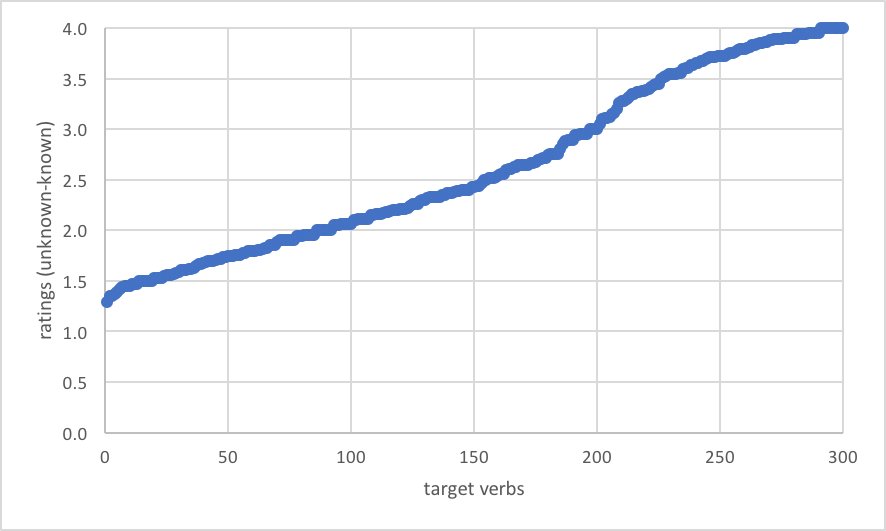
\includegraphics[width=.9\linewidth]{figures/dataset_neo_ratings.png}
\end{figure}

\begin{figure}[htbp]
  \caption{Unknown/known target particle verbs across domains.}
  \label{fig:neo-ratings-domain}
  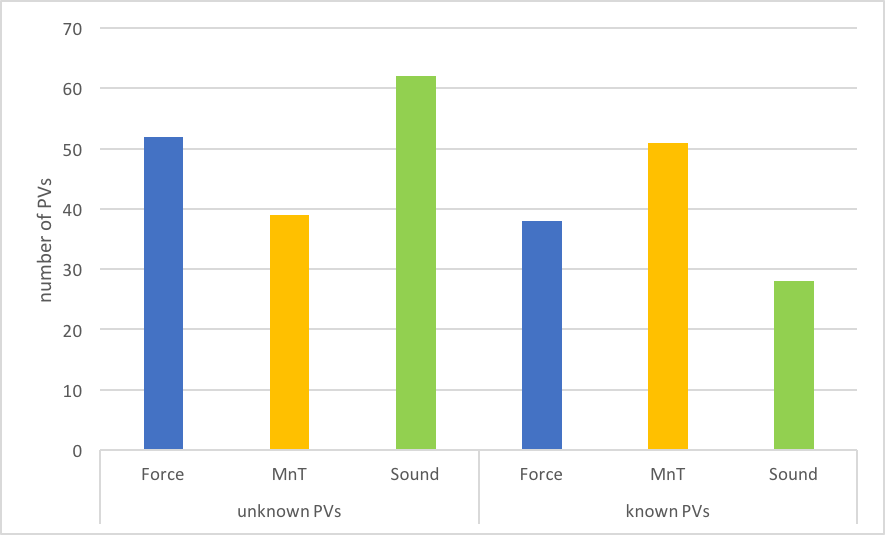
\includegraphics[width=.9\linewidth]{figures/dataset_neo_domain_ratings.png}
\end{figure}


%\clearpage
\subsubsection{Concept image selection across particles}

The heat map in Figure~\ref{fig:particle-prop} shows the preferences
for selected concept images across particle types, calculated as
follows. For each annotated verb instance we determined the proportion
of selection for each concept image. For example, if two concept
images were chosen by a specific participant and for a specific verb
instance, each of the two concept images received a proportion of 0.5,
and all others received proportions of 0. These proportions were then
averaged over all PV instances with the same particle type, across
participants. The color red indicates strong preferences of a specific
concept image selected for a specific particle type, the color blue
indicates weak preferences. Overall, the average preferences range
from 0.004 to 0.214.

\begin{figure}[htbp]
  \centering
  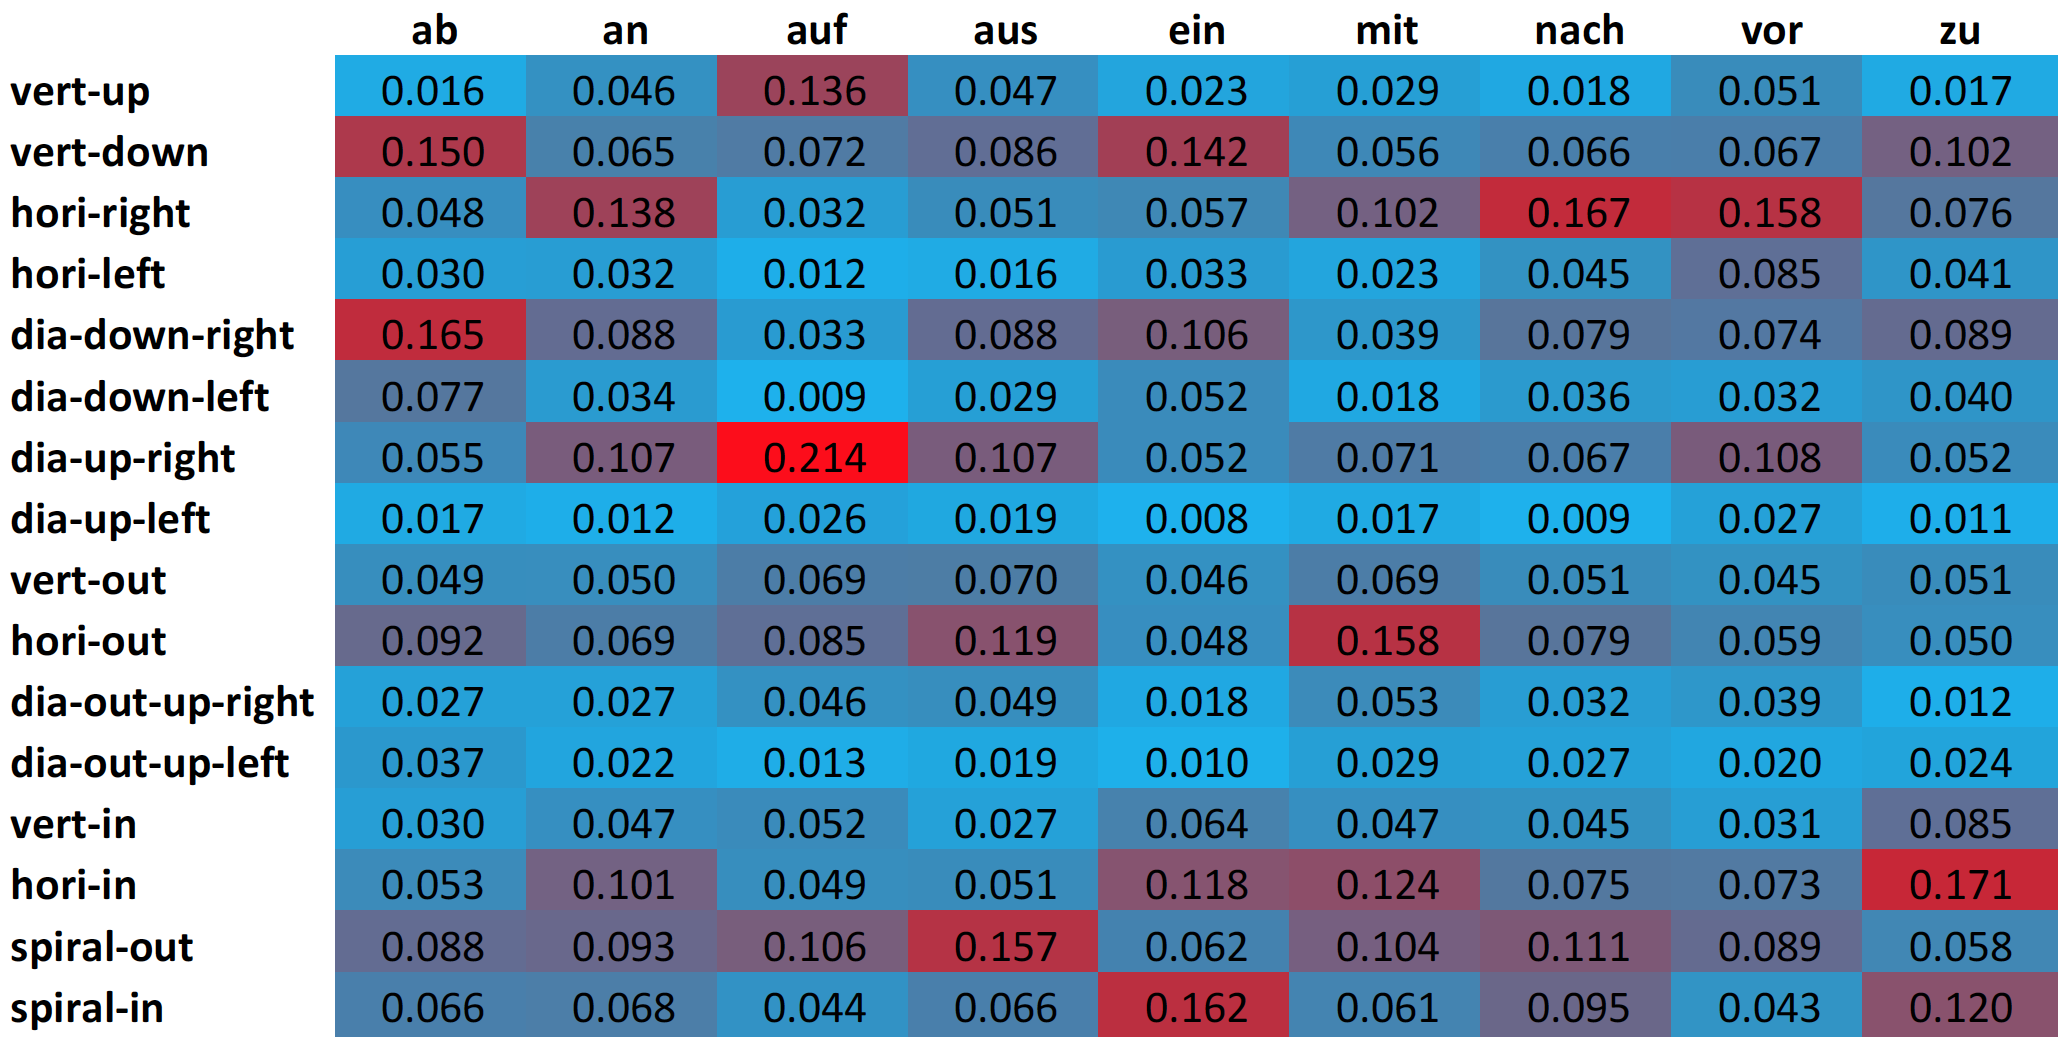
\includegraphics[width=\linewidth]{figures/dataset_particles_heat2}
  \caption{Concept image selection across particle types.}
  \label{fig:particle-prop}
\end{figure}

\clearpage
The heat map demonstrates that the particles exhibit clearly different
concept image profiles. The particle \textit{auf}, for example, achieved the
overall strongest preference of 0.214 for the concept image
\textci{dia-up-right}, and a preference of 0.136 for
\textci{vert-up}. \textit{ab} shows preferences of $\ge$0.150 for the
concepts \textci{dia-down-right} and \textci{vert-down}. \textit{an},
\textit{nach} and \textit{vor} are associated most strongly with
\textci{hori-right} (preferences 0.138--0.167), \textit{aus} with
\textci{spiral-out} (preference 0.157), \textit{ein} with
\textci{spiral-in} and \textci{vert-down} (preferences 0.162 and
0.142, respectively), \textit{mit} with \textci{hori-out} (preference
0.158), and \textit{zu} with \textci{hori-in} (preference 0.171).


%\clearpage
\subsubsection{Concept image selection across existing PVs and PV neologisms}

The heat maps in Figure~\ref{fig:particle-prop-neo} specify the
particle selections of concept images from Figure~\ref{fig:particle-prop}
regarding the participants' ratings of PV knowledge. That is, the
upper plot in Figure~\ref{fig:particle-prop-neo} shows concept image preferences
across particles for well-known PVs with an average rating $\ge$2.5,
and the lower plot shows concept image preferences across particles for rather
unknown PVs with an average rating $<$2.5.

\begin{figure}[htbp]
  \caption{Concept image selection across particles and (un)known PVs.}
  \label{fig:particle-prop-neo}
  % The figures (un)known were put into a heat map together, rather
  % than separately.
% 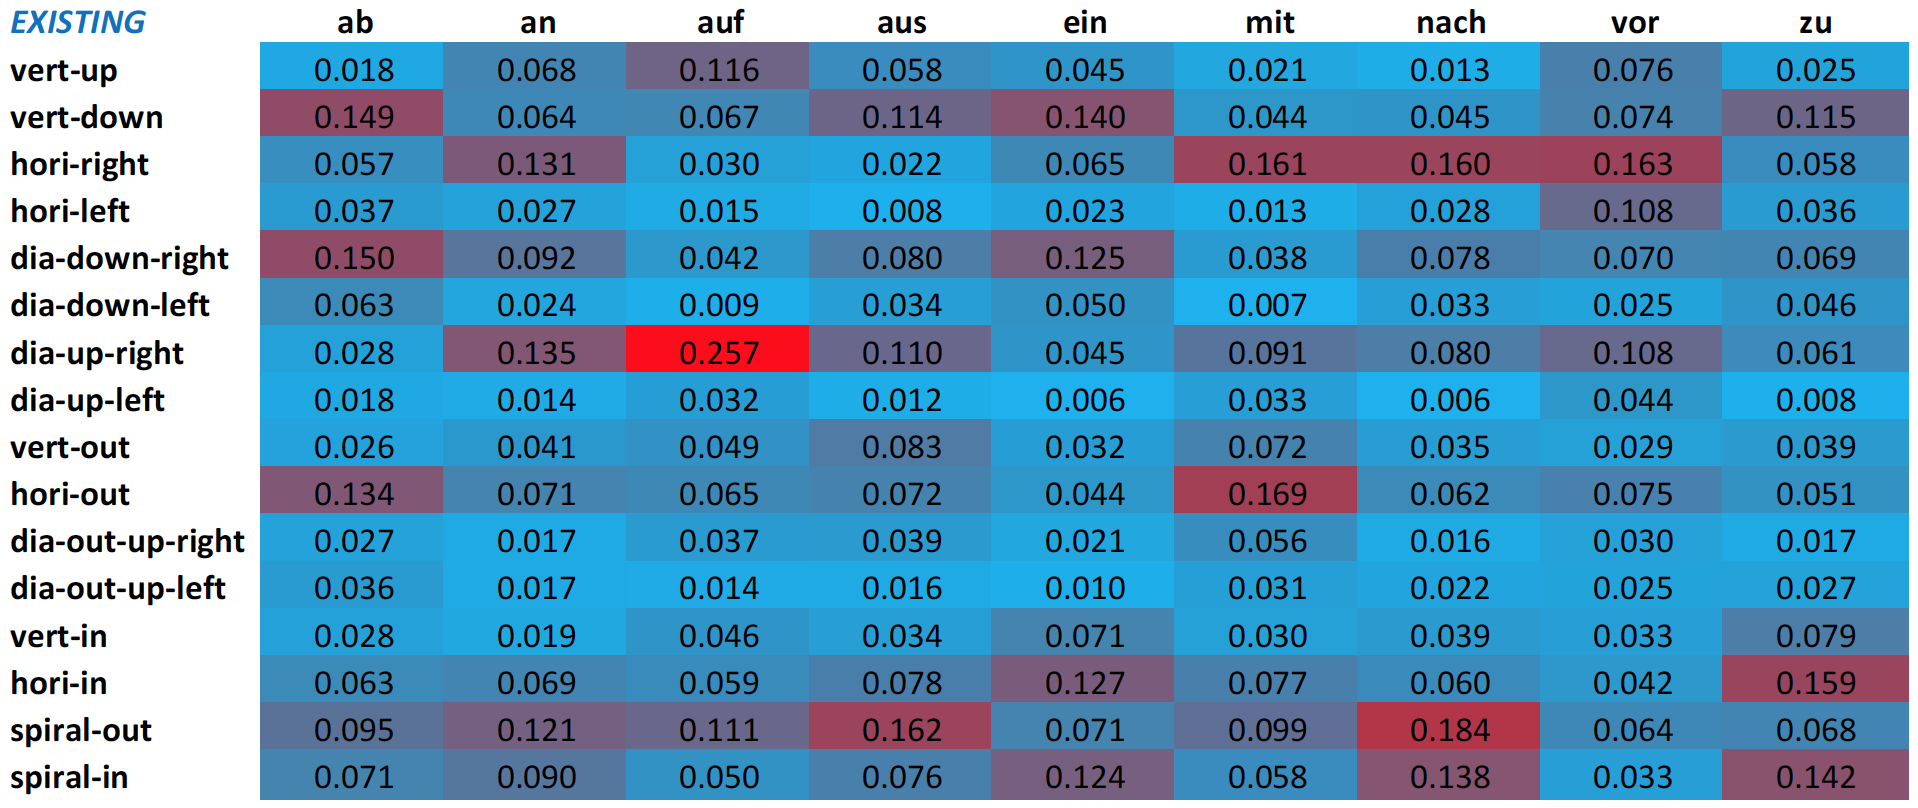
\includegraphics[width=\linewidth]{figures/dataset_particles_neoNO}
  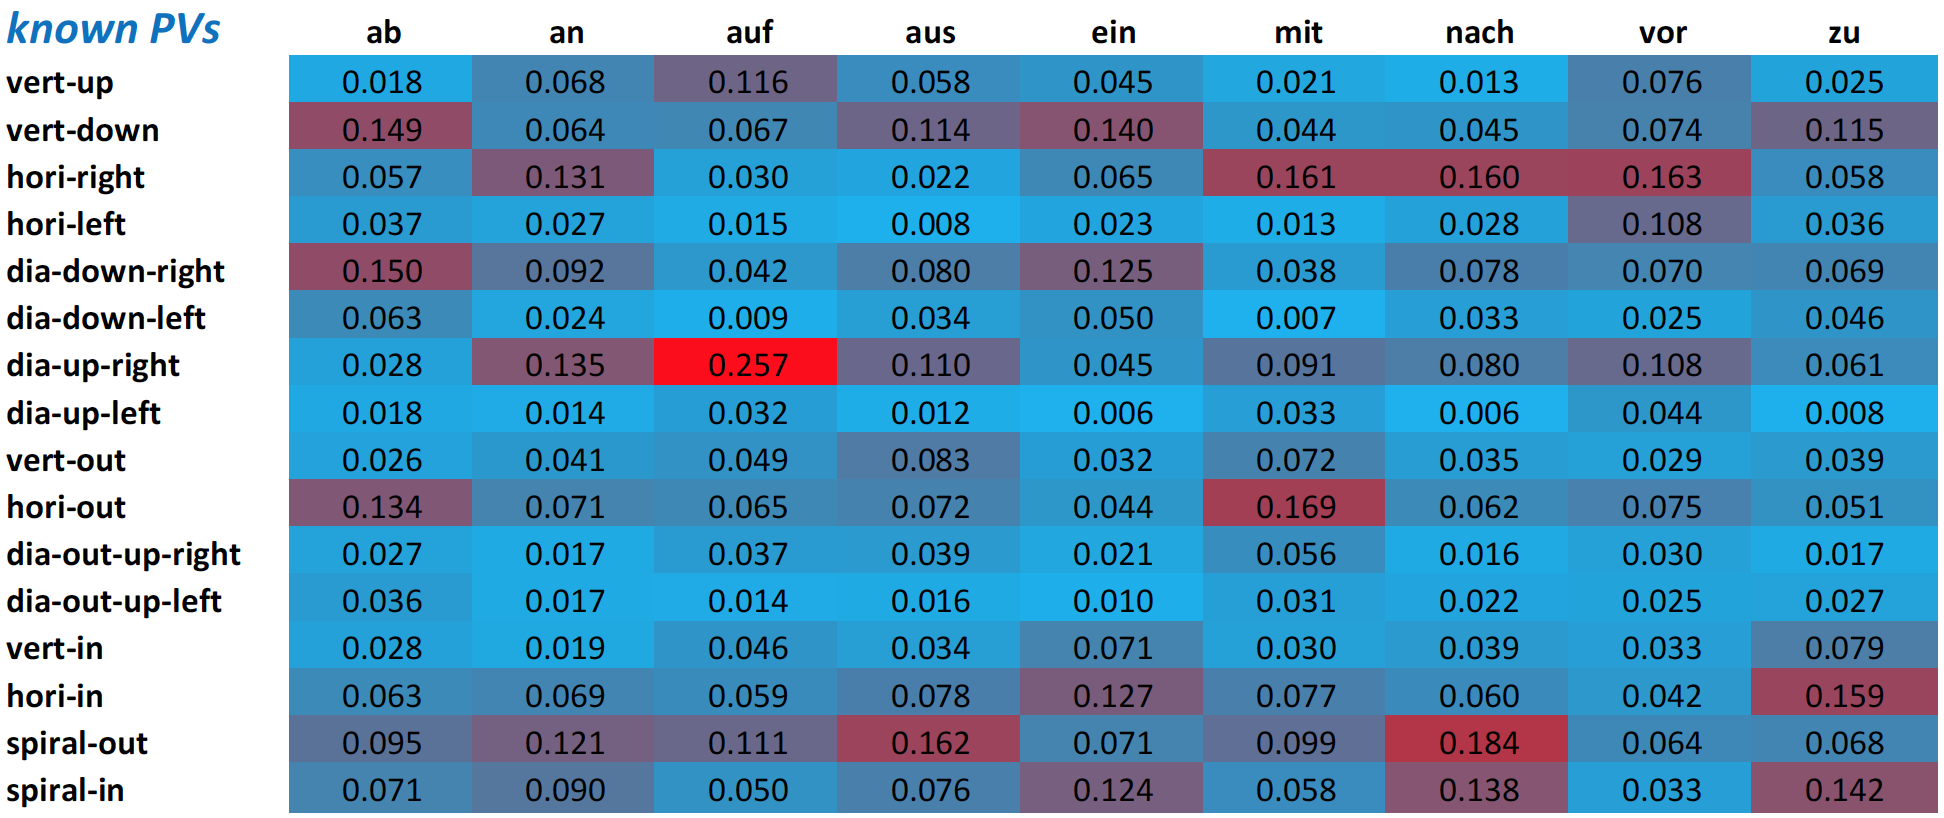
\includegraphics[width=\linewidth]{figures/dataset_particles_known}
  \vspace{+4mm}\\
  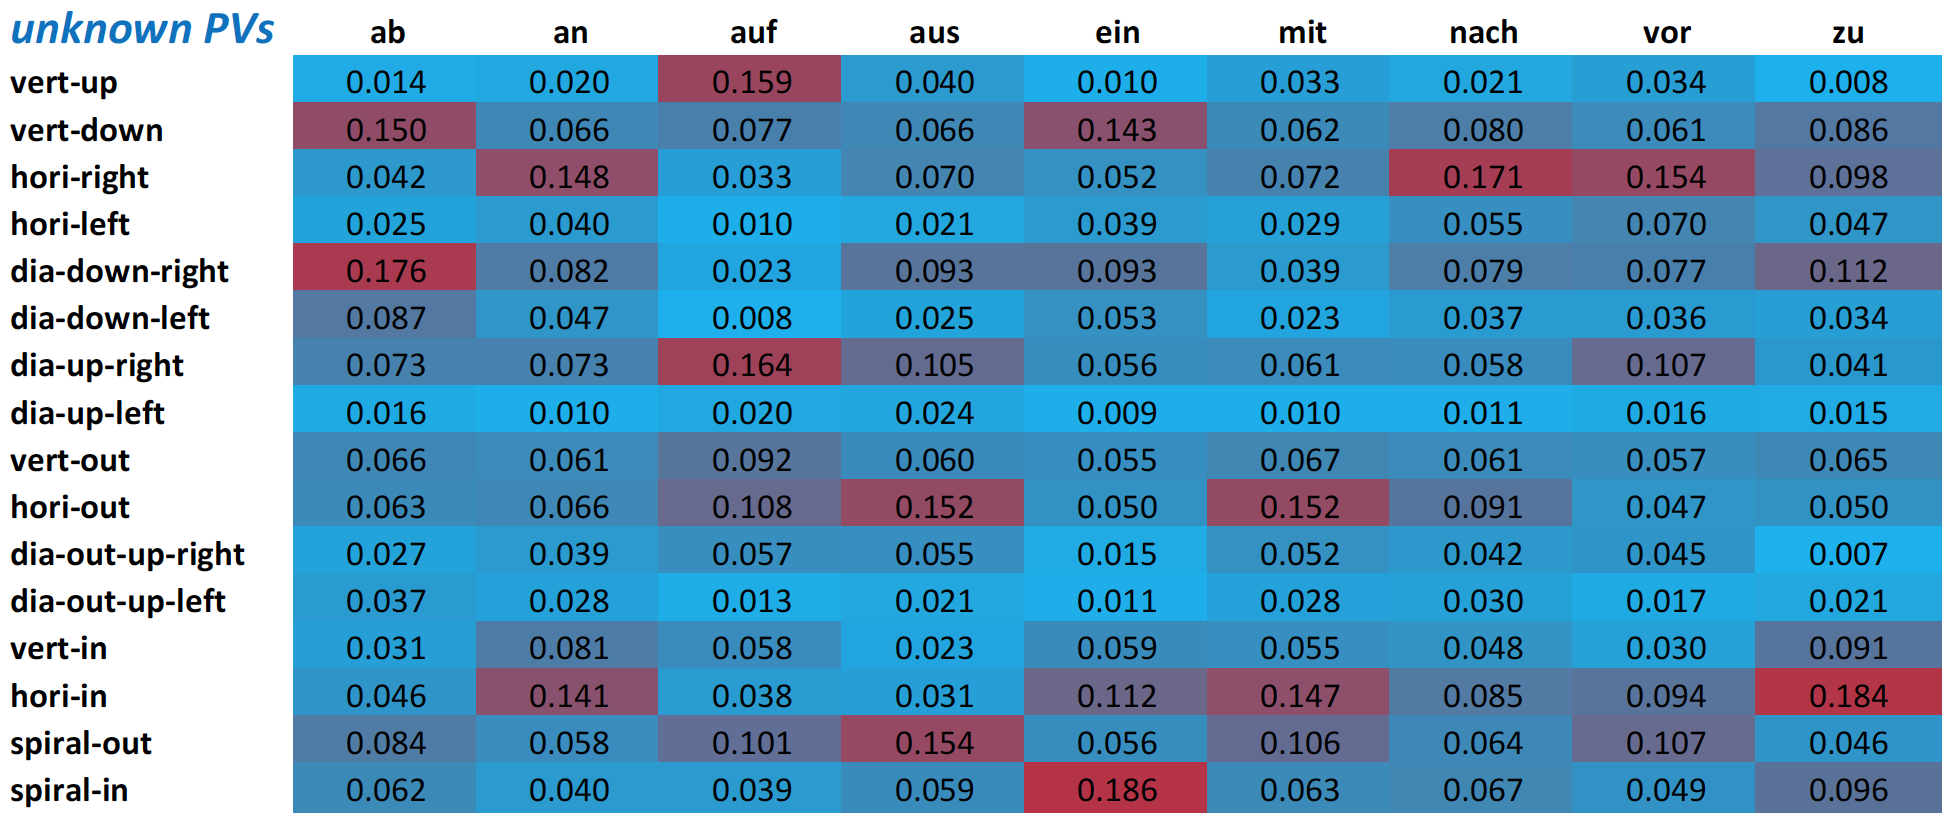
\includegraphics[width=\linewidth]{figures/dataset_particles_unknown}
%  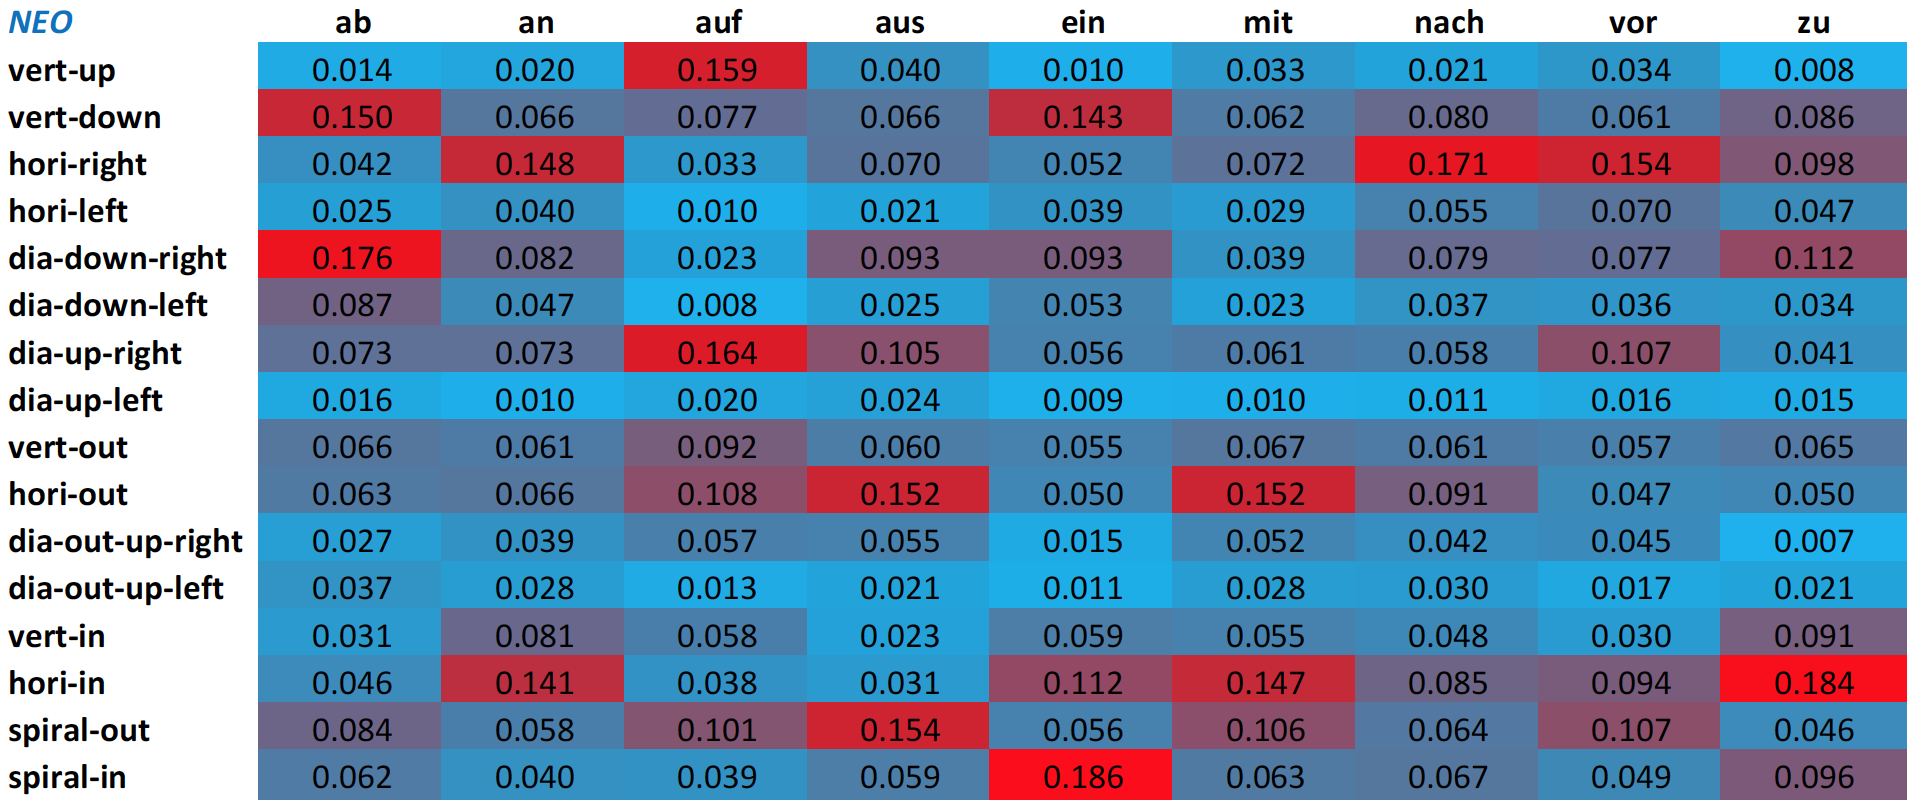
\includegraphics[width=\linewidth]{figures/dataset_particles_neoYES}
\end{figure}

While we expected to see more strongly associated concept images for
particles in rather unknown PVs (refering to some predominant meaning
contribution(s)), this is the case for the majority of particle types
(e.g., \textci{dia-down-right} for \textit{ab}; \textci{hori-right}
and \textci{hori-in} for \textit{an}; \textci{spiral-in} for
\textit{ein}; \textci{hori-right} for \textit{nach} and \textit{vor};
\textci{hori-in} for \textit{zu}) but not for \textit{auf, aus} and
\textit{mit}. The figure however indicates that the concept image
selections are largely stable for well-known vs. unknown particle
verbs, i.e., the strongest preferences of particle types regarding
concept images show up in both heat maps.


\subsubsection{Concept image selection across BV source domains}

Figures~\ref{fig:BV-prop-domain} and~\ref{fig:particle-prop-domain}
look into concept image selection across BV source
domains. Figure~\ref{fig:BV-prop-domain} presents the average
preferences of selected concept images per domain across all particle
types. It shows that already the base verbs exhibit clearly different
concept image profiles when taking into account the respective source
domain. For \texttt{Force} BVs, the inward-pointing concept images
\textci{hori-in} (0.221) and \textci{vert-in} (0.125) received the
strongest preferences; for \texttt{MnT} BVs, the concept image
\textci{vert-down} (0.154) received the predominant amount of
selections, followed by a set of concept images with preferences of
$\approx$0.100--0.110: \textci{spiral-out}, \textci{vert-out},
\textci{dia-down-right} and \textci{hori-out}, thus favouring
downward- and outward-pointing arrow types while being rather
flexible, i.e., with less strong overall preferences; for
\texttt{Sound} BVs, the strongly favoured concept image is
\textci{spiral-out} (0.288), with a set of secondary selections for
\textci{hori-out} (0.134), \textci{spiral-in} (0.109) and
\textci{vert-out} (0.097), thus favouring spiral-shaped and
outward-directed arrows.

\begin{figure}[htbp]
  \caption{Concept image selection across base verbs, with reference to their domains.}
  \label{fig:BV-prop-domain}
  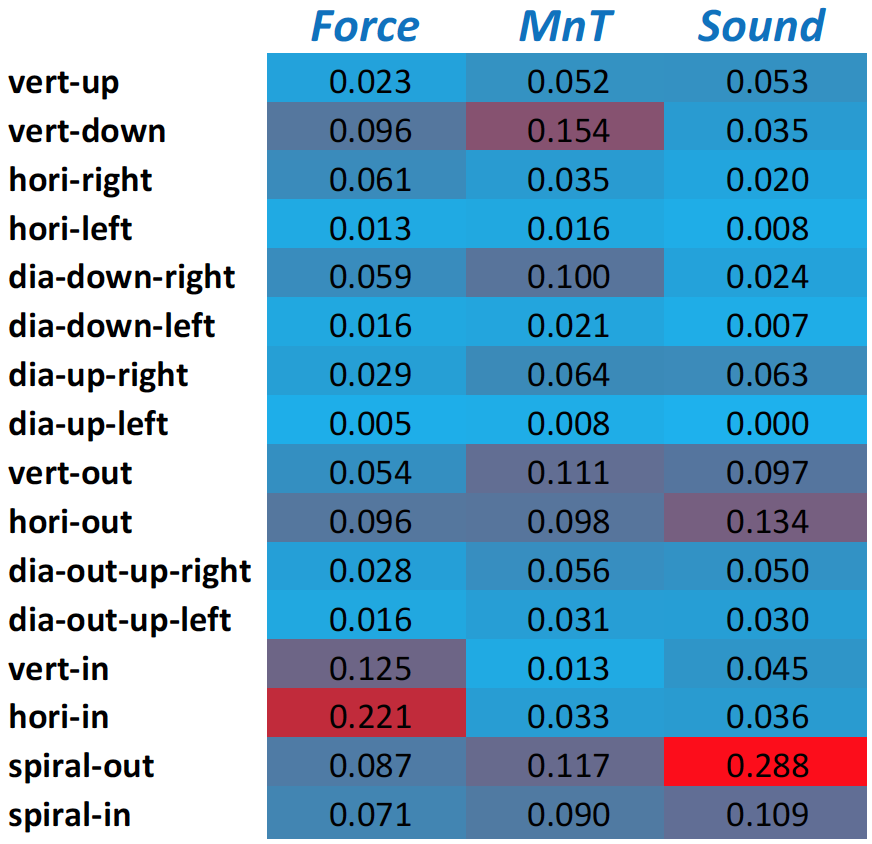
\includegraphics[width=0.55\linewidth]{figures/dataset_particles_domains_BVs}
\end{figure}

Figure~\ref{fig:particle-prop-domain} demonstrates that the BV
patterns across concept images are partly preserved and partly
over-written when combining the BVs with specific particles. PVs
composed of \texttt{Force} BVs and particles \textit{an, ein, mit, zu}
inherit the strong preference for \textci{hori-in}. Similarly, PVs
composed of \texttt{Sound} BVs and particles \textit{aus, ein, mit,
  nach, zu} inherit the strong preferences for spirals from the BVs,
with \textit{an, nach, vor} at the same time showing strong
preferences for \textci{hori-right}. For PVs composed of \texttt{MnT}
BVs, where already the concept image preferences for the BVs were less
skewed than for the other two domains, it seems that also the
respective PVs do not exhibit specific domain-dependent concept image
preferences.

\begin{figure}[htbp]
  \caption{Concept image selection across particles and BV domains.}
  \label{fig:particle-prop-domain}
  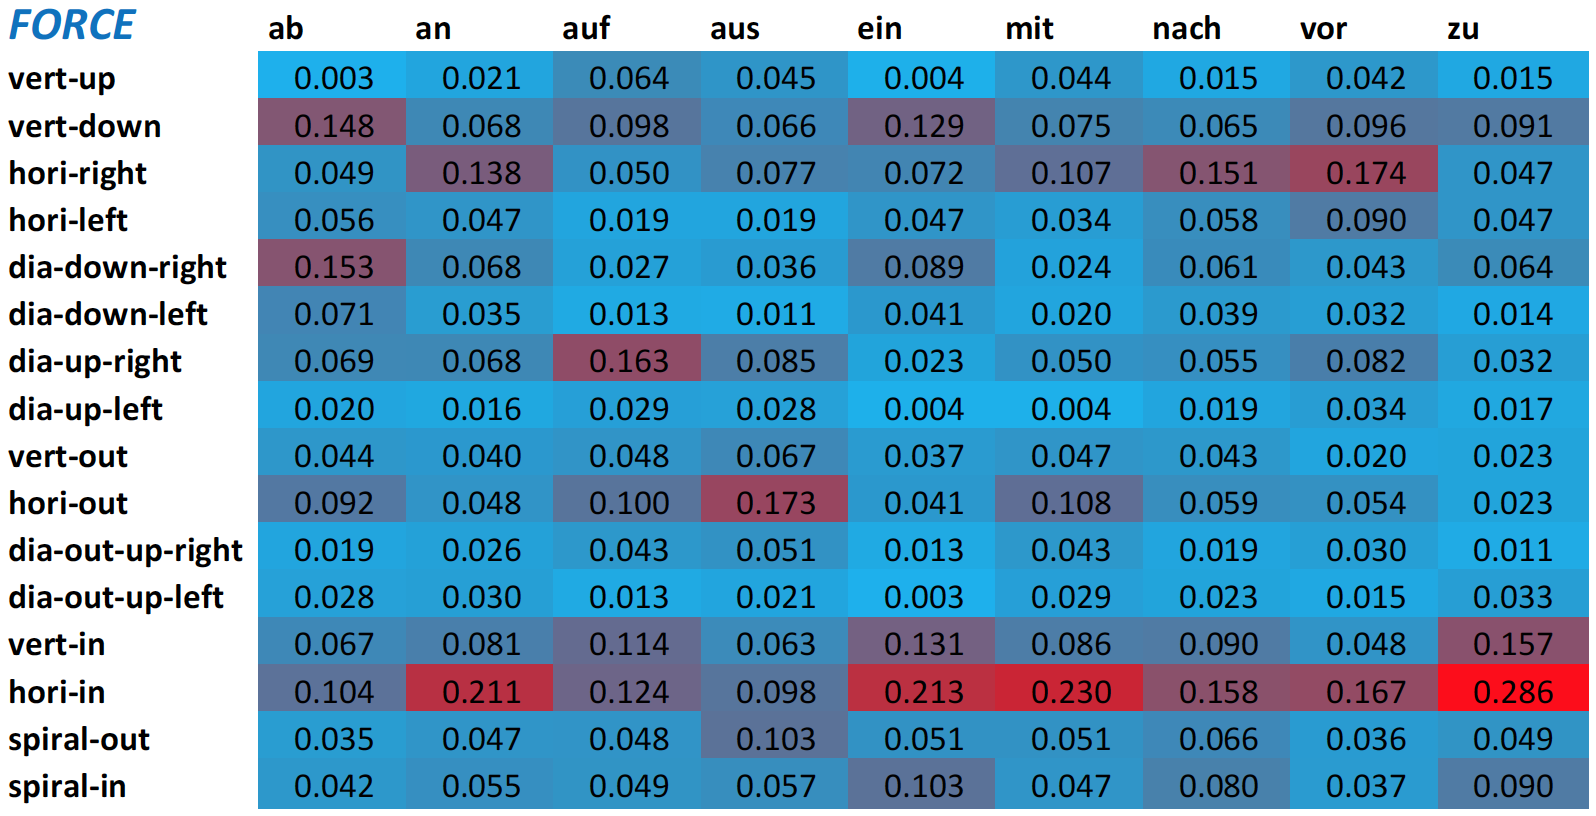
\includegraphics[width=0.9\linewidth]{figures/dataset_particles_domains_force}
  \vspace{+2mm}\\
  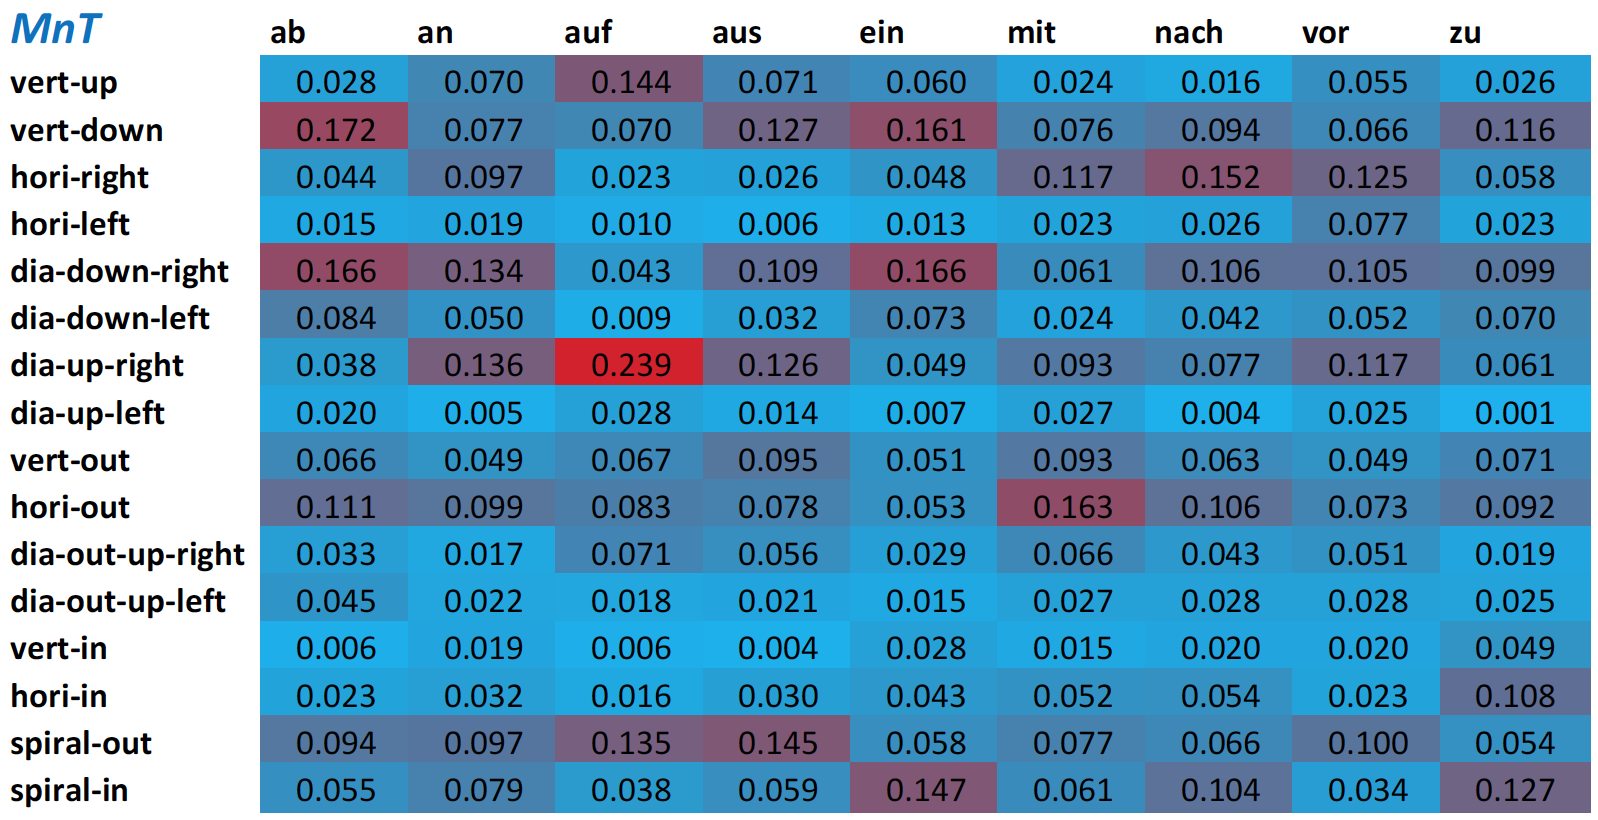
\includegraphics[width=0.9\linewidth]{figures/dataset_particles_domains_mnt}
  \vspace{+2mm}\\
  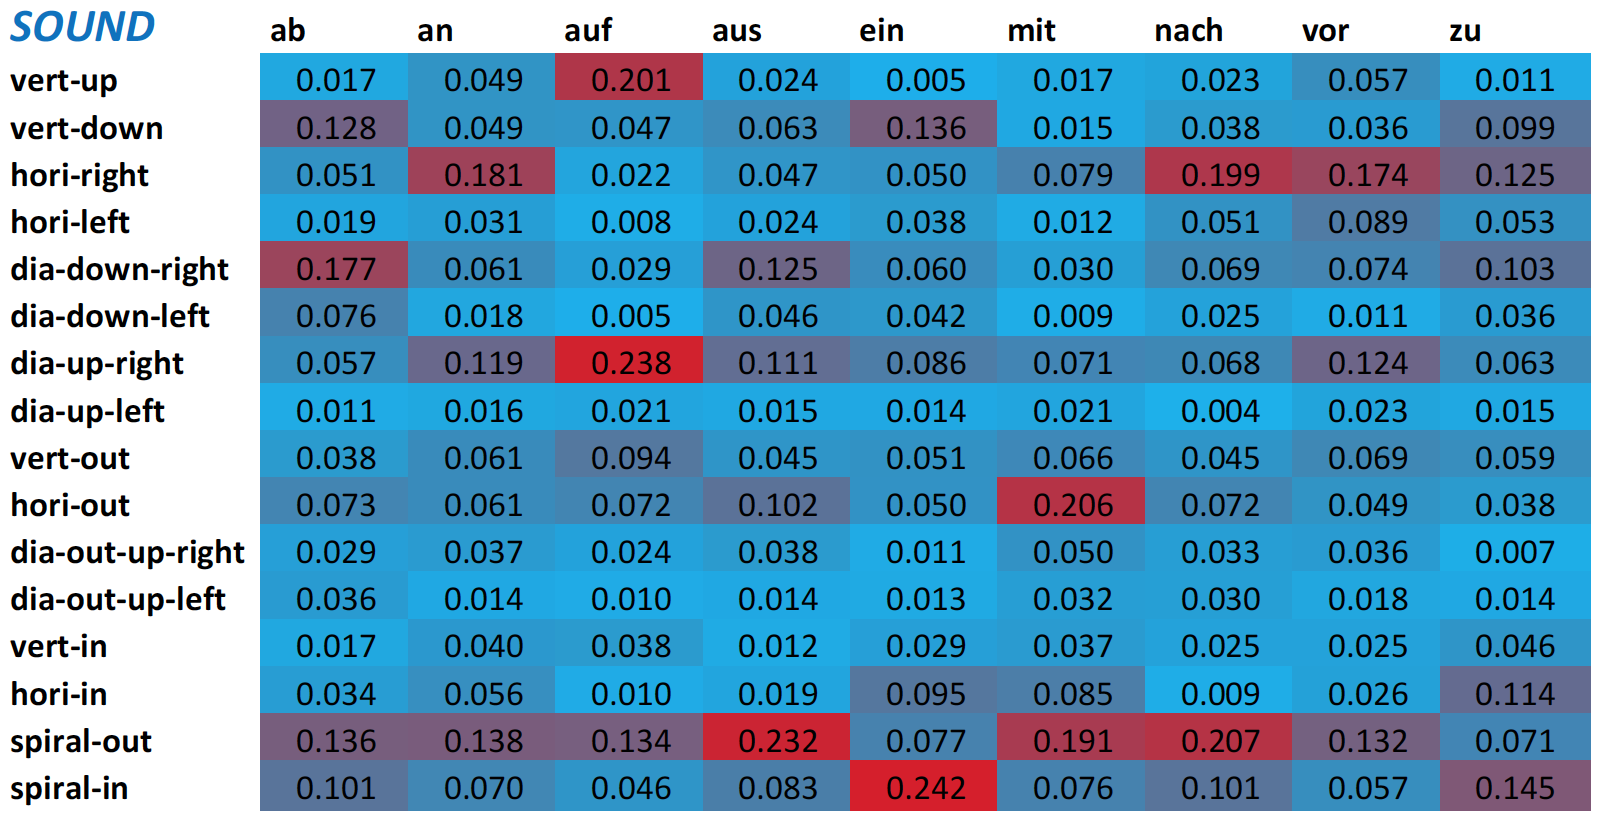
\includegraphics[width=0.9\linewidth]{figures/dataset_particles_domains_sound}
\end{figure}

%\clearpage
Across domains, the PVs with particles \textit{ab, auf, nach, vor}
appear to contribute rather constant meaning components: the most
strongly selected concept images tend to be consistent across BV source domains
and largely correspond to the overall strongest concept images in
Figure~\ref{fig:particle-prop}. PVs with particles \textit{an} and
\textit{auf} represent constants in a different way: in comparison to
the other particle types, they seem to be more flexible in their
meaning contribution, i.e., they do not show particularly strong
preferences for specific concept images but similarly strong preferences for a
range of concept images.  Nevertheless, also these more constant particle
meanings are influenced by the BV domains; for example, \textit{ab}
shows a strong preference for \textci{spiral-out} when combined with
\texttt{Sound} BVs; \textit{an} shows a strong preference for
\textci{hori-in} when combined with \texttt{Force} BVs; \textit{auf}
shows a strong preference for \textci{vert-up} when combined with
\texttt{Sound} BVs and only a loose preference for
\textci{dia-up-right} when combined with \texttt{Force} BVs;
\textit{nach} and \textit{vor} show strong preferences for spirals
when combined with \texttt{Sound} BVs and no strong preferences when
combined with \texttt{MnT} BVs.


\clearpage
\section{Discussion}
\label{sec:2discussion}

In the remainder of this article, we refer the analyses in the
previous section back to our hypotheses about particle meanings and
particle concepts (Section~\ref{sec:disc-general}) before we explore
the role of the BV source domains (Section~\ref{sec:disc-domain}) and
go into detailed meaning investigations regarding the particle
\textit{ab} (Section~\ref{sec:disc-ab}).

\subsection{General analysis of particle concept hypotheses}
\label{sec:disc-general}

The experiment participants associated \textit{auf} and \textit{ab}
with the vertical arrows (\textci{vert-up} and \textci{vert-down}) and
also with the corresponding diagonal versions pointing to the right:
\textci{dia-up-right} and \textci{dia-down-right}, as predicted. The
respective diagonal arrows pointing to the left were not chosen, which
is an indication for the involvement of the horizontal time dimension.
%
The particle \textit{an} was, as predicted, most strongly associated
with the \textci{hori-right} concept image; the additionally predicted
\textci{dia-up-right} concept image achieved a secondary preference.\footnote{Our
  results regarding \textit{auf} and \textit{an} are also in
  accordance with the insights of a lexical decision experiment
  presented by \cite{FrassinelliEtAl:17}, which indicated that the
  particles have a predominant vertical/horizontal directionality,
  respectively.}
%
\textit{nach} and \textit{vor} were strongly associated with the
\textci{hori-right} concept image, which again indicates a reference to the time
dimension. Since most \textit{nach} and \textit{vor} readings have a
temporal component, a derivation of the basic particle concept from
the time domain instead of the space domain should therefore be
considered as an explanation.

In the case of \textit{aus}, the \textci{spiral-out} concept image was selected
most often. This can be explained by the strong association of the
particle's prevalent meaning refering to a \textit{container} Image
Schema necessary for assigning a direction to \textit{aus}. Since this
experimental concept image setting consisted only of two-dimensional arrows, we
can however only speculate about the relevance of the container
representation. In contrast, \textit{ein} was --in accordance with our
assumptions-- associated with \textci{vert-down} (next to
\textci{spiral-in}), although these directions also require the notion
of a container. In order to conceptualise an outside area, as
necessary for many \textit{aus} PV readings, it might be sufficient to
think of a single wall in order to distinguish between an outside and
an inside area. This could explain why \textit{ein} received --in
contrast to \textit{aus}, stronger preferences for the predicted concept images
based on the constraint of the existence of an imaginary container.

The particle \textit{mit} was most strongly associated with the
\textci{hori-out} concept image, in accordance with our assumptions. \textit{zu}
was not linked to \textci{dia-up-right}, which we considered as
possible concept representation for the intentional readings with an
abstract goal. The strongest selection was in favour of the
double-arrow concept image \textci{hori-in}, followed by \textci{spiral-in}, thus
suggesting that a different sense of the particle was more salient in
the contexts of the selected BVs. For example, for the PVs
\textit{zuzerren} (`to drag until closed') and \textit{zustopfen} (`to
plug') the particle introduces a closure relation, which is connected
to the also chosen \textci{vert-down}. However, the \textit{zu}-PVs
based on the abstract \texttt{Sound} BVs were also associated with
these concept images, which at first sight does not fit to the concrete closure
notion. Here, it seems to be more likely that the selection for
\textci{spiral-in} does not represent the particle meaning, but the
meanings of the \texttt{Sound} BVs. Together with the choice of
\textci{hori-in} as in \textit{zudröhnen} ([\textit{zu}]+`to drone/get
stoned'), this points to an interpretation of \textit{zu} as an
abstract closure, where the closure is understood as the impairment of
auditory perception, as realised through the very dominant and
constant sound provided by the BV \textit{dröhnen}. In this
interpretation, each arrow head of \textci{hori-in} conceptually
points to one ear.

\subsection{Analysis of BV source domains}
\label{sec:disc-domain}

Figure~\ref{fig:BV-prop-domain} suggested that the BV source domains
were associated with different preferences for concept images,
although none of the BV classes is directional from a lexical semantic
perspective. We believe that the associations between source domains
and concept images thus indicate conceptual relations to
directionality.

The \texttt{MnT} domain with its concrete BVs provides strong
preferences for the concepts \textci{vert-down},
\textci{dia-down-right}, \textci{vert-out}, \textci{hori-out} and
\textci{spiral-out}. The associations with \textci{hori-out} and
\textci{spiral-out} can be explained with the visually clearly defined
and easily imaginable manners of movement of the BVs
\textit{schleifen} (`to sand'), \textit{sägen} (`to saw'),
\textit{spitzen} (`to sharpen'), etc., whereas the associations to
\textci{vert-down}, \textci{vert-out} and \textci{dia-down-right} can
be traced back to the manners of movements of \textit{hämmern} (`to
hammer'), \textit{graben} (`to dig'), \textit{schaufeln} (`to
shovel'), etc. However, the question arises why only the
downward-pointing concept images were chosen and not the upward-oriented ones. We
approach the question on a theoretical semantic basis. The BVs are
denominal action verbs, either derived from an instrument (such as a
shovel, a hammer, a fork) or from an intended result (such as a
grave), and describe a repetitive motion. The involved motion has at
least two changes of directions, marking the extreme points of the
movement. The direct objects of \texttt{MnT} verbs typically refer to
one of those extreme points, as in example~(\ref{ex:schaufelGraben}),
where \textit{schaufeln} refers to the area beneath the ground which
lies below our usual perceptual horizon. This idea corresponds to
\cite{LachmairEtAl:16}'s research which shows that words trigger
specific spatial locations. Other frequent arguments of
\textit{schaufeln}, such as \textit{hole} and \textit{soil}, also
refer to such a ``down'' area, as in examples~(\ref{ex:schaufelLoch})
and~(\ref{ex:schaufelErde}). Here, the motion is spanned between the
initial position of the instrument and the position of the affected
area. In the
examples~(\ref{ex:schaufelGraben})--(\ref{ex:schaufelErde}), the
direction of the shovel motion is defined between the initial ``up''
location of the shovel and the ``down'' location of the ground, thus
justifying the downward concept images over upward concept images.

\ea\label{ex:schaufelGraben} 
\gll Karin schaufelt einen Graben.\\ 
Karin shovel a graben\\
\glt `Karin shovels a graben.'
\z 

\ea\label{ex:schaufelLoch} 
\gll Karin schaufelt ein Loch.\\ 
Karin shovel a hole\\
\glt `Karin shovels a hole.'
\z  

\ea\label{ex:schaufelErde} 
\gll Karin schaufelt Erde.\\ 
Karin shovel soil\\
\glt `Karin shovels soil.'
\z

On the contrary, the \texttt{Sound} BVs, which are the most abstract
verbs in this data set, were not linked to many of our simple
directional concept images. They were mainly associated with the spirals, thus
suggesting a mental mapping to the prototypical picture of a sound
wave. That is, the underlying idea of the spiral as concept
representation was a uniform expansion, which matches to the motion
behaviour of sound waves. In addition, there was some preference for
the double-headed arrows \textci{hori-out} and \textci{vert-out} as
concept images for the BVs with a repetitive sound character. This can be
attributed to the strongly prototypical manner of sound production
actions, which are usually caused by an up-and-down motion as in
drumming, or a left-to-right motion as in clapping. This means that
the \texttt{Sound} BVs, which are not directional from a lexical
semantic perspective, were analysed as conceptually directional. This
clear-cut mapping between spiral and sound wave as well as between
double-headed arrow and manner-of-production of repetitive sounds,
allows distinguishing between the concept images triggered by the BVs and the concept images
triggered by the particle, which provides insight into the composition
process and explains the low compatibility between particle types and
\texttt{Sound} BVs, as reflected in the high number of neoPVs in
Figure~\ref{fig:neo-ratings-domain}.

The \texttt{Force} BVs describe events which are mainly defined
through the interplay of two concrete arguments. In comparison to
\texttt{MnT} verbs, the \texttt{Force} verbs are less concrete, but at
the same time they are also less abstract than the \texttt{Sound}
verbs. The importance of the arguments shows up in the preference for
the concepts \textci{hori-in} and \textci{vert-in}, which both have
two arrow heads. The concept images are thereby similar to the vectors used in
the schematic representations of forceful verbs by \cite{Zwarts:10}.
% The preferred association of \texttt{Force} BVs with
% \textci{vert-down} can be explained by the negative connotation of
% forces in their most common contexts with a power inequality, and
% therefore also with suppression as a result.

\subsection{Analysis of particle \textit{ab}}
\label{sec:disc-ab}

In the last part of our analyses we focus on concept image preferences
regarding one specific particle type. We choose \textit{ab}, the
particle which is strongly associated with a downward direction.

Figure \ref{fig:particle-prop-domain-ab} shows the distribution over
concept images for PVs with particle \textit{ab} across BV source
domains. In all three domains, the participants agreed on the two
\textsc{Down} concepts (i.e., \textci{vert-down} and
\textci{dia-down-right}), although the PVs in the experiment were
assigned to different lexical semantic classes by \cite{Kliche:11}.

\begin{figure}[htbp]
  \caption{Concept image selection for \textit{ab} across BV domains.}
  \label{fig:particle-prop-domain-ab}
  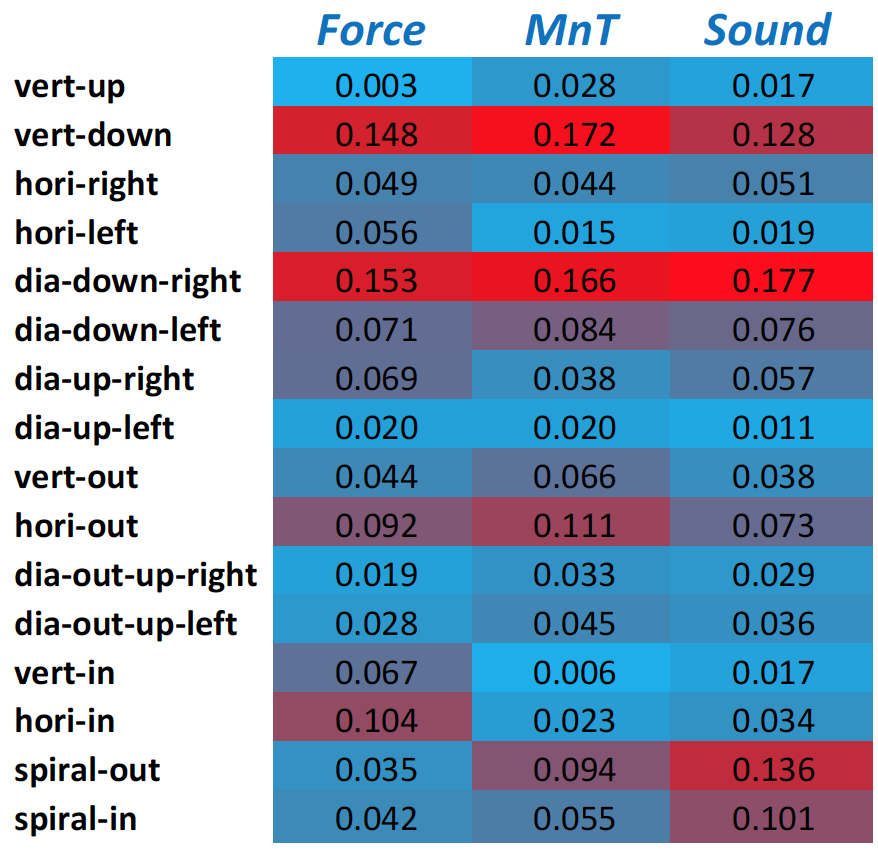
\includegraphics[width=0.55\linewidth]{figures/dataset_particles_domains_ab}
\end{figure}

Looking into specific PVs with strong preferences for the two
\textsc{Down} concept images, an example instance of an unknown PV is represented
by \textit{abhämmern} ([ab]+`to hammer'),
cf. example~\ref{ex:abhaemmern}. We assume that this PV was understood
as a separation performed by a hammering force. \textit{abquetschen}
(`to squeeze off') in example~(\ref{ex:abquetschen}) is an instance of
a well-known PV where the particle is combined with a \texttt{Force}
BV, describing a force that causes a \textsc{Separation}. The
well-known PV \textit{abklingen} combines the particle with a
\texttt{Sound} BV; literally, it describes that a sound fades away,
but it is more common in its metaphorical reading of approaching the
end of an event together with a value decrease, as in
example~(\ref{ex:abklingenSturm}). The approaching of the end of the
storm can be conceptualised as decreasing intensity within both the
value and the time dimensions, or can alternatively be interpreted
only temporal, as a slowly ending process. However, in comparison to
the previous examples no causer is involved, suggesting that the
downward meaning is conceptually connected to \textit{ab}, even if
from a lexical semantic perspective only the result is expressed.

\ea\label{ex:abhaemmern}
\gll Karin hämmert den rostigen Nagel ab.\\
Karin hammer the rusty nail [ab]\\
\glt `Karin detaches the rusty nail by hammering.'
\z

% \ea\label{ex:abschalten}
% \gll Karin schaltet die Waschmaschine ab.\\
% Karin switch the {washing machine} [ab]\\
% \glt `Karin switches off the washing machine.'
% \z

\ea\label{ex:abquetschen}
\gll Karin hat sich ihren Finger abgequetscht.\\
Karin has herself her finger [ab]+squeeze\\
\glt `Karin has crushed her finger.'
\z

\ea \label{ex:abklingenSturm}
\gll Der Sturm klingt ab.\\
The storm sound [ab]\\
\glt `The storm is about to stop.'
\z

The examples illustrate that even though the contexts are rather
different, the meanings of the particle can in all cases be traced
back to a downward direction, either causing or be caused by a
separation, varying according to the constraints. We argue that the
downward concept is not only the basic meaning component, but the
prototypical reading for the particle \textit{ab}.


\section{Conclusion}

In this article, we have shown that directional concepts, visually
represented as arrow pictographs, can be applied to a systematically
composed set of German particle verbs and their underlying base
verbs. Furthermore, the selected concept images were mostly in
accordance with the particle directions predicted on the basis of
example sentences, lexical-semantic classifications and spatial
experience, and largely stable for well-known vs. unknown particle
verbs. Thus, direction is a concept that should be taken into account
as a part of the PV composition process and the contribution of the
particle to the particle verb meaning.

Understanding potential particle fundamentals as concepts, instead of
meanings, has the advantage that senses are not considered as
discrete, static classifications requiring plenty of compromises or
borderline cases. Concepts as basic components are flexible and can
easily be adjusted to various contexts. Thereby, classes of similar
contextual requirements trigger similar concept adjustments, and hence
are assumed to enforce a specific particle sense.


%\clearpage
%\section*{Abbreviations}
%
%\begin{table}
%  \label{tab:abbrev}
%
%  \centering
%  \begin{tabular}{ll}
%
%    BV & base verb \\
%    MnT & Machines and Tools \\
%    neoPV & PV neologism \\
%    PV & particle verb \\
%
%  \end{tabular}
%\end{table}


\section*{Acknowledgements}

The research was supported by the DFG Collaborative Research Centre
SFB 732 (Sylvia Springorum, Sabine Schulte im Walde) and the DFG
Heisenberg Fellowship SCHU-2580/1 (Sabine Schulte im Walde).


% Bibliography:

\vspace{+5mm}
{\sloppy
  \printbibliography[heading=subbibliography,notkeyword=this]
}


\clearpage
\section*{Appendix}

\begin{table}
  \caption{Selected 30 base verbs and their source domains. All these
    base verbs were systematically composed to a total of 270 particle
    verbs by prefixing them with the nine constituent particle types
    \textit{ab, an, auf, aus, ein, mit, nach, vor, zu}.}
  \label{tab:bv-sd}

  \centering
  \begin{tabular}{ll}

    Base verb & Source domain \\ \hline

    biegen & Force \\
    brechen & Force \\
    brummen & Sound \\
    donnern & Sound \\
    drängen & Force \\
    dröhnen & Sound \\
    gabeln & Machines and Tools \\
    graben & Machines and Tools \\
    heulen & Sound \\
    hämmern & Machines and Tools \\
    jaulen & Sound \\
    klappern & Sound \\
    klingen & Sound \\
    kämmen & Machines and Tools \\
    pressen & Force \\
    quetschen & Force \\
    rattern & Sound \\
    schalten & Machines and Tools \\
    schaufeln & Machines and Tools \\
    schleifen & Machines and Tools \\
    schrauben & Machines and Tools \\
    spitzen & Machines and Tools \\
    stauen & Force \\
    stopfen & Force \\
    summen & Sound \\
    sägen & Machines and Tools \\
    wummern & Sound \\
    zerren & Force \\
    zwingen & Force \\
    zwängen & Force \\

  \end{tabular}
\end{table}


\end{document}
